\section{Windows Server 2019}

\subsection{Ajout de fonctionnalités de Windows Server}

\begin{itemize}
    \item Démarrer la machine virtuelle Windows Server;
    \item Ouvrir le gestionnaire de serveur (s'ouvre normalement automatiquement lors du démarrage de la machine);
    \item Cliquer sur "\textit{Ajouter des rôles et des fonctionnalités}" (figure \ref{Funcs_WinS/1});
    \item Aller dans la section \textbf{Avant de commencer}, puis cliquer sur \textit{Suivant} (figure \ref{Funcs_WinS/2});
    \item Aller dans la section \textbf{Type d'installation}, sélectionner la première option, puis cliquer sur \textit{Suivant} (figure \ref{Funcs_WinS/3});
    \item Aller dans la section \textbf{Sélection du serveur}. Cocher l'option "Sélectionner un serveur de pool de serveurs". Choisir \textit{DC01.EPITAF.lab}, puis cliquer sur \textit{Suivant} (figure \ref{Funcs_WinS/4});
    \item Aller dans la section \textbf{Rôles de serveurs}. Cocher les options :
    \begin{itemize}
        \item Serveur DHCP (installé);
        \item Serveur DNS (installé);
        \item Services AD DS (Installé).
    \end{itemize}
    Cliquer sur \textit{Suivant} (figure \ref{Funcs_WinS/5});
    \item Aller dans la section \textbf{Sélection des fonctionnalités}. Cliquer sur \textit{Installer} (figure \ref{Funcs_WinS/6}).
\end{itemize}

\begin{figure}[h!]
	\begin{center}
		\caption{Ouverture de la fenêtre d'ajout de rôles et des fonctionnalités de windows server}
		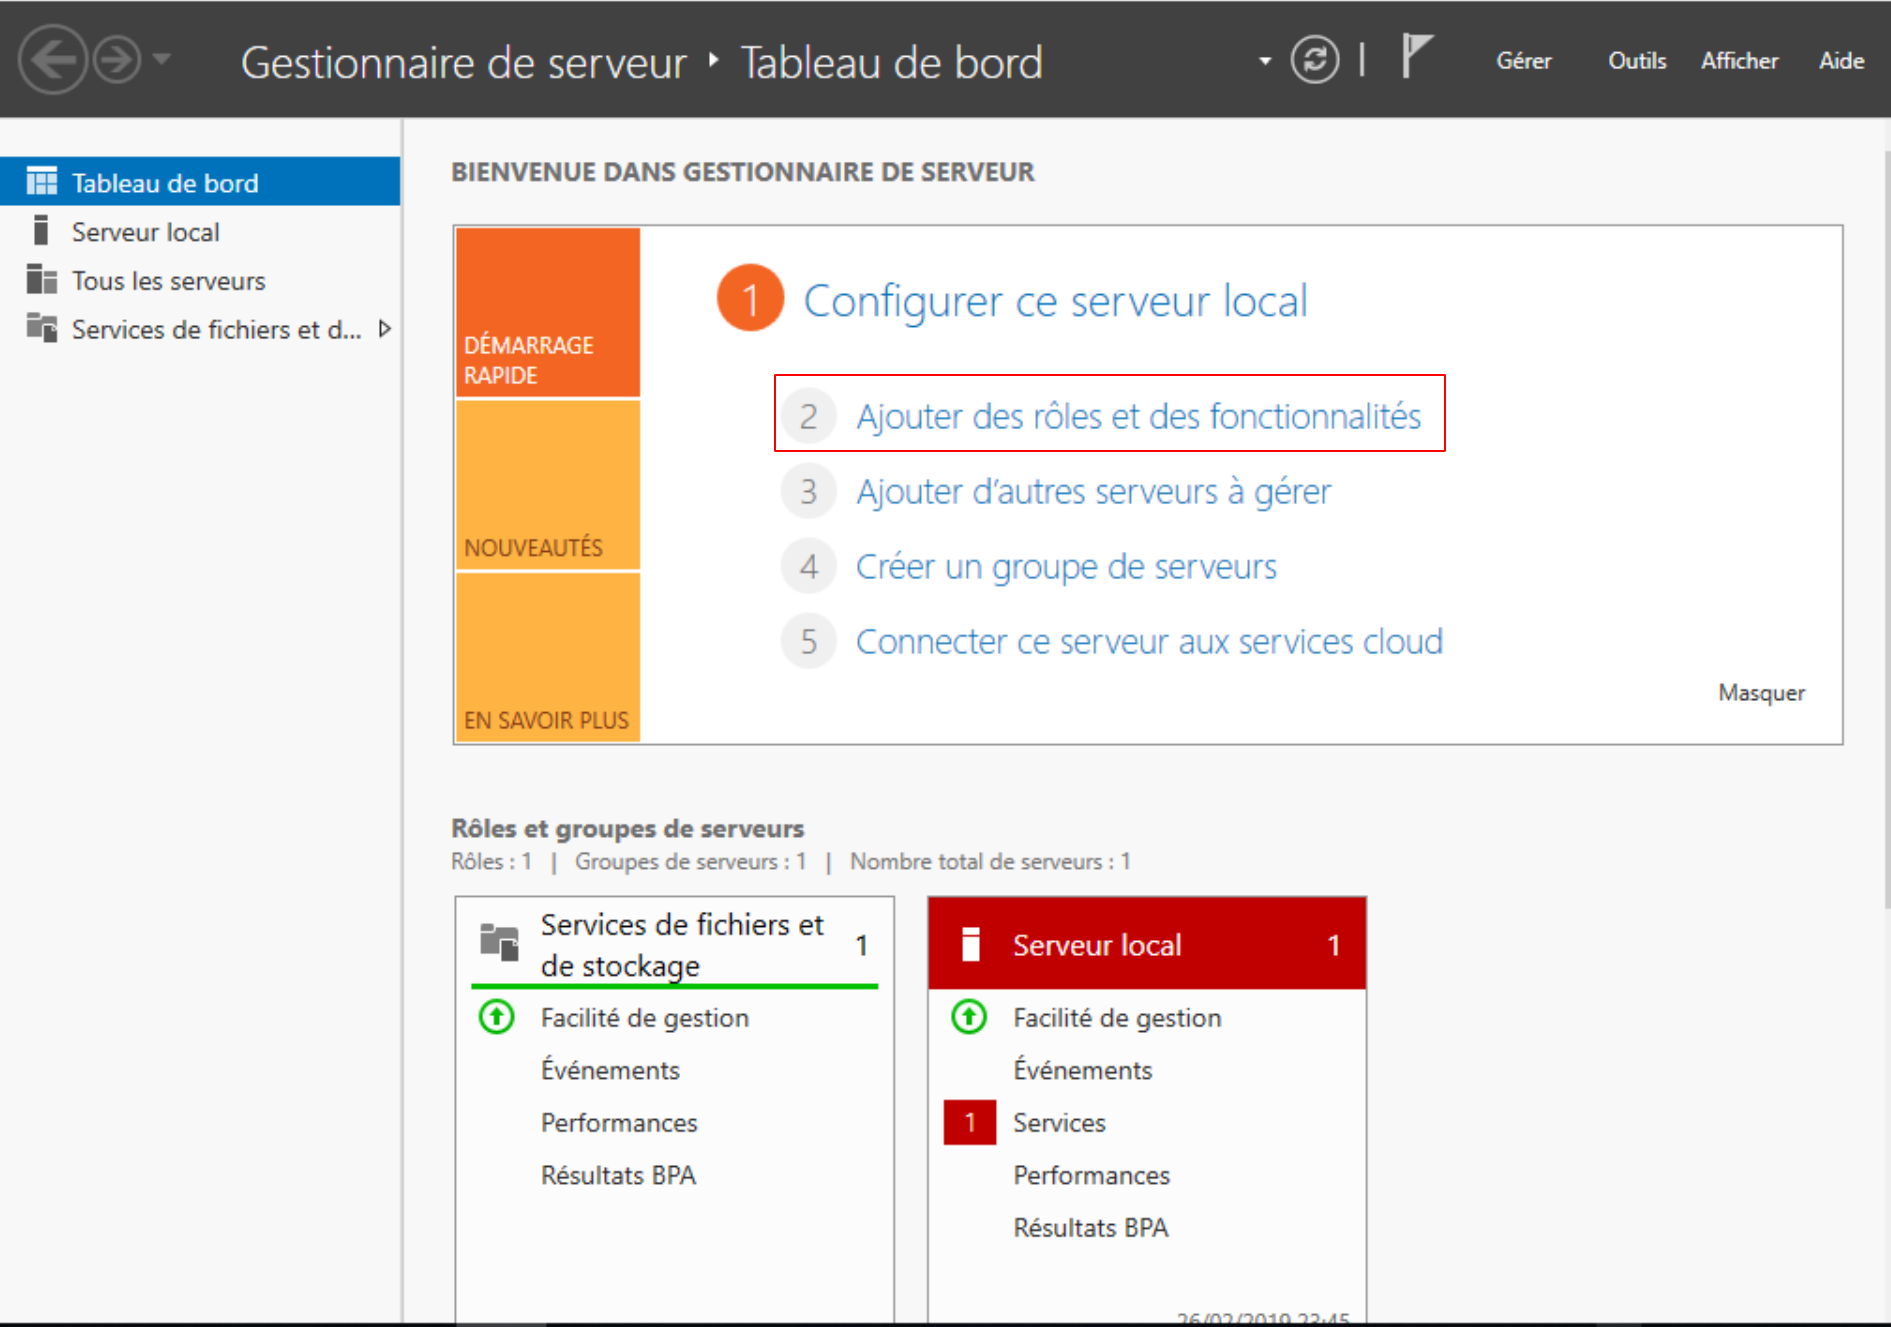
\includegraphics[scale=0.7]{WS_Screenshots/29.png}
		\label{Funcs_WinS/1}
	\end{center}
\end{figure}
\FloatBarrier
    

\begin{figure}[h!]
	\begin{center}
		\caption{Avant de commencer - Rôles et fonctionnalités de windows server}
		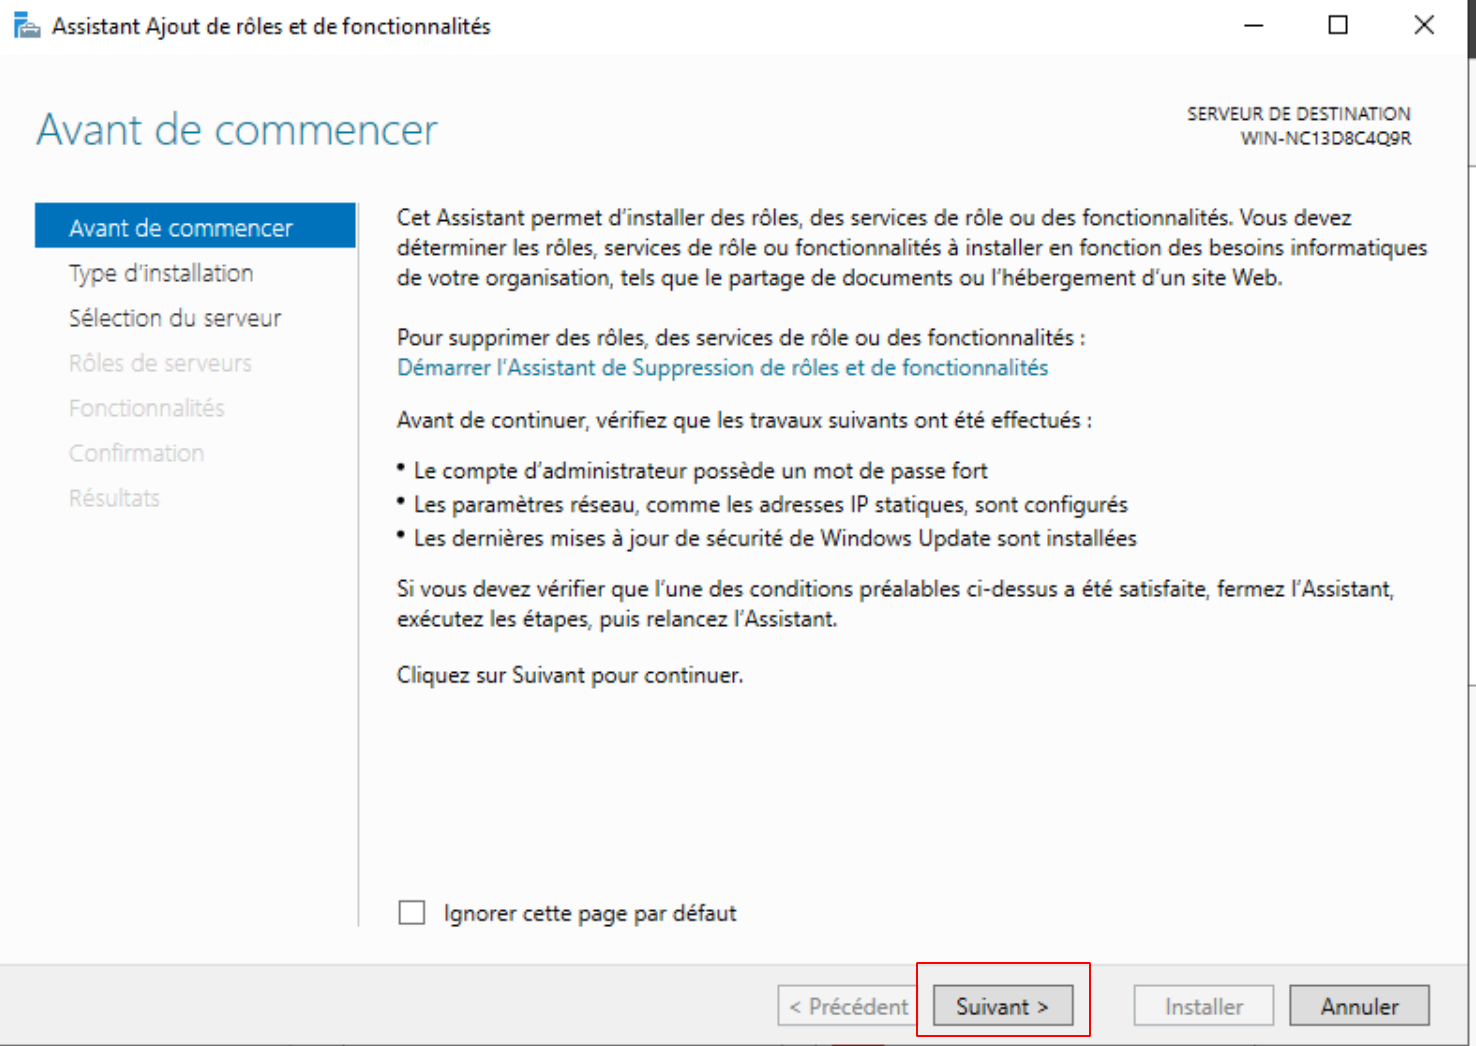
\includegraphics[scale=0.7]{WS_Screenshots/30.png}
		\label{Funcs_WinS/2}
	\end{center}
\end{figure}
\FloatBarrier 
    

\begin{figure}[h!]
	\begin{center}
		\caption{Type d'installation - Rôles et fonctionnalités de windows server}
		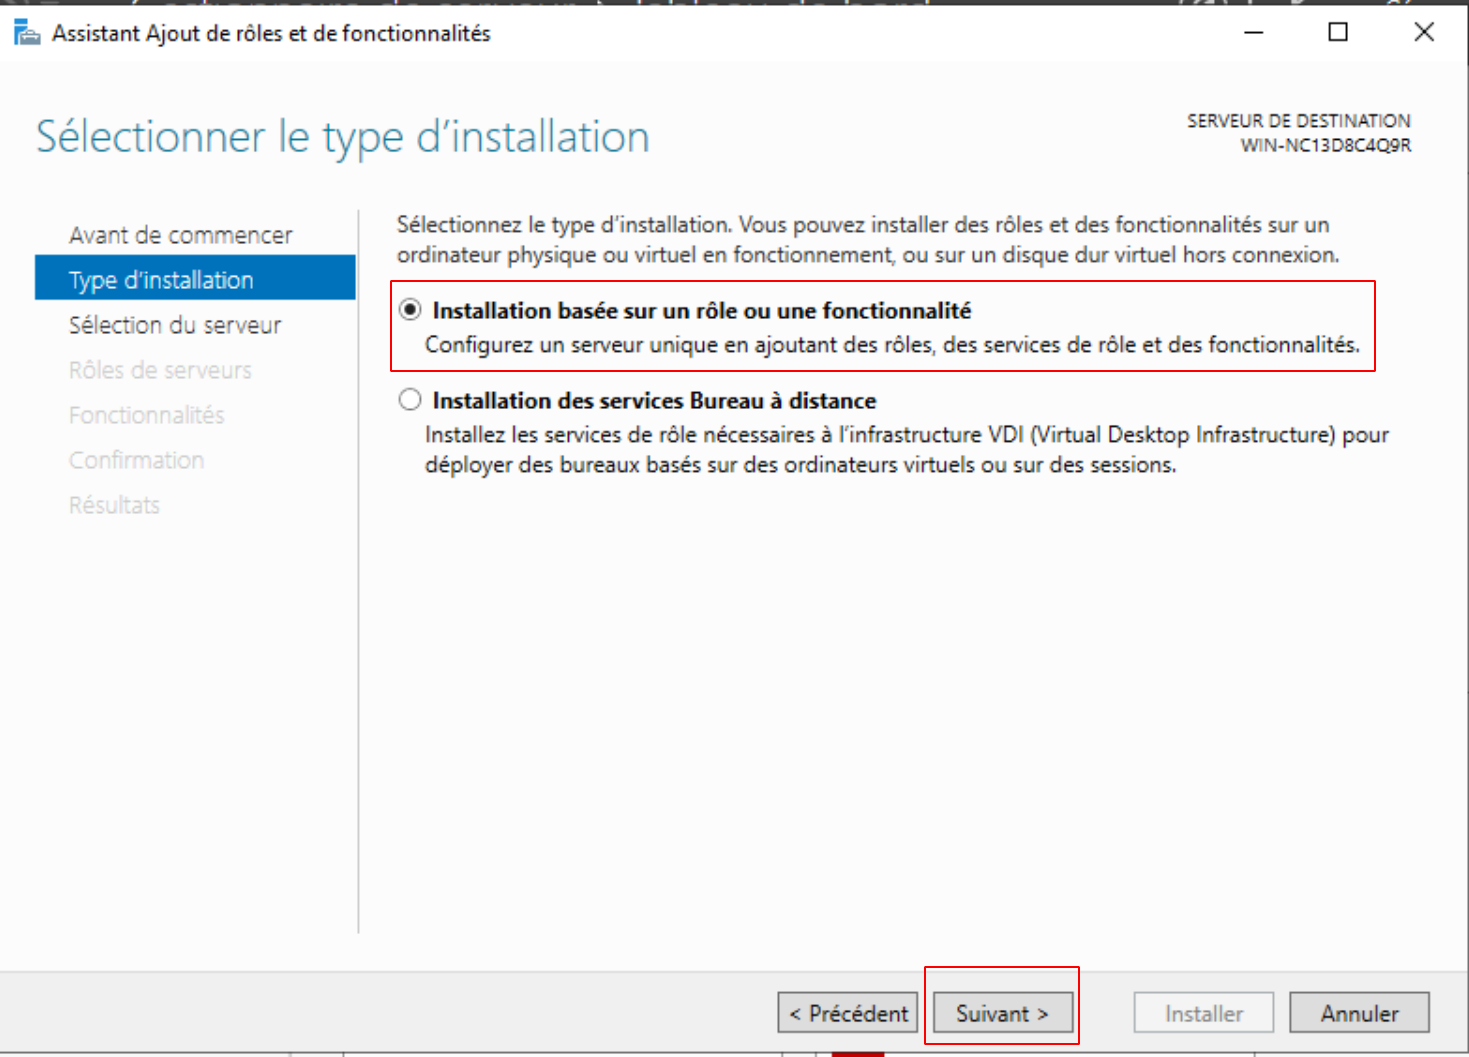
\includegraphics[scale=0.7]{WS_Screenshots/31.png}
		\label{Funcs_WinS/3}
	\end{center}
\end{figure}
\FloatBarrier 
    

\begin{figure}[h!]
	\begin{center}
		\caption{Sélection du serveur - Rôles et fonctionnalités de windows server}
		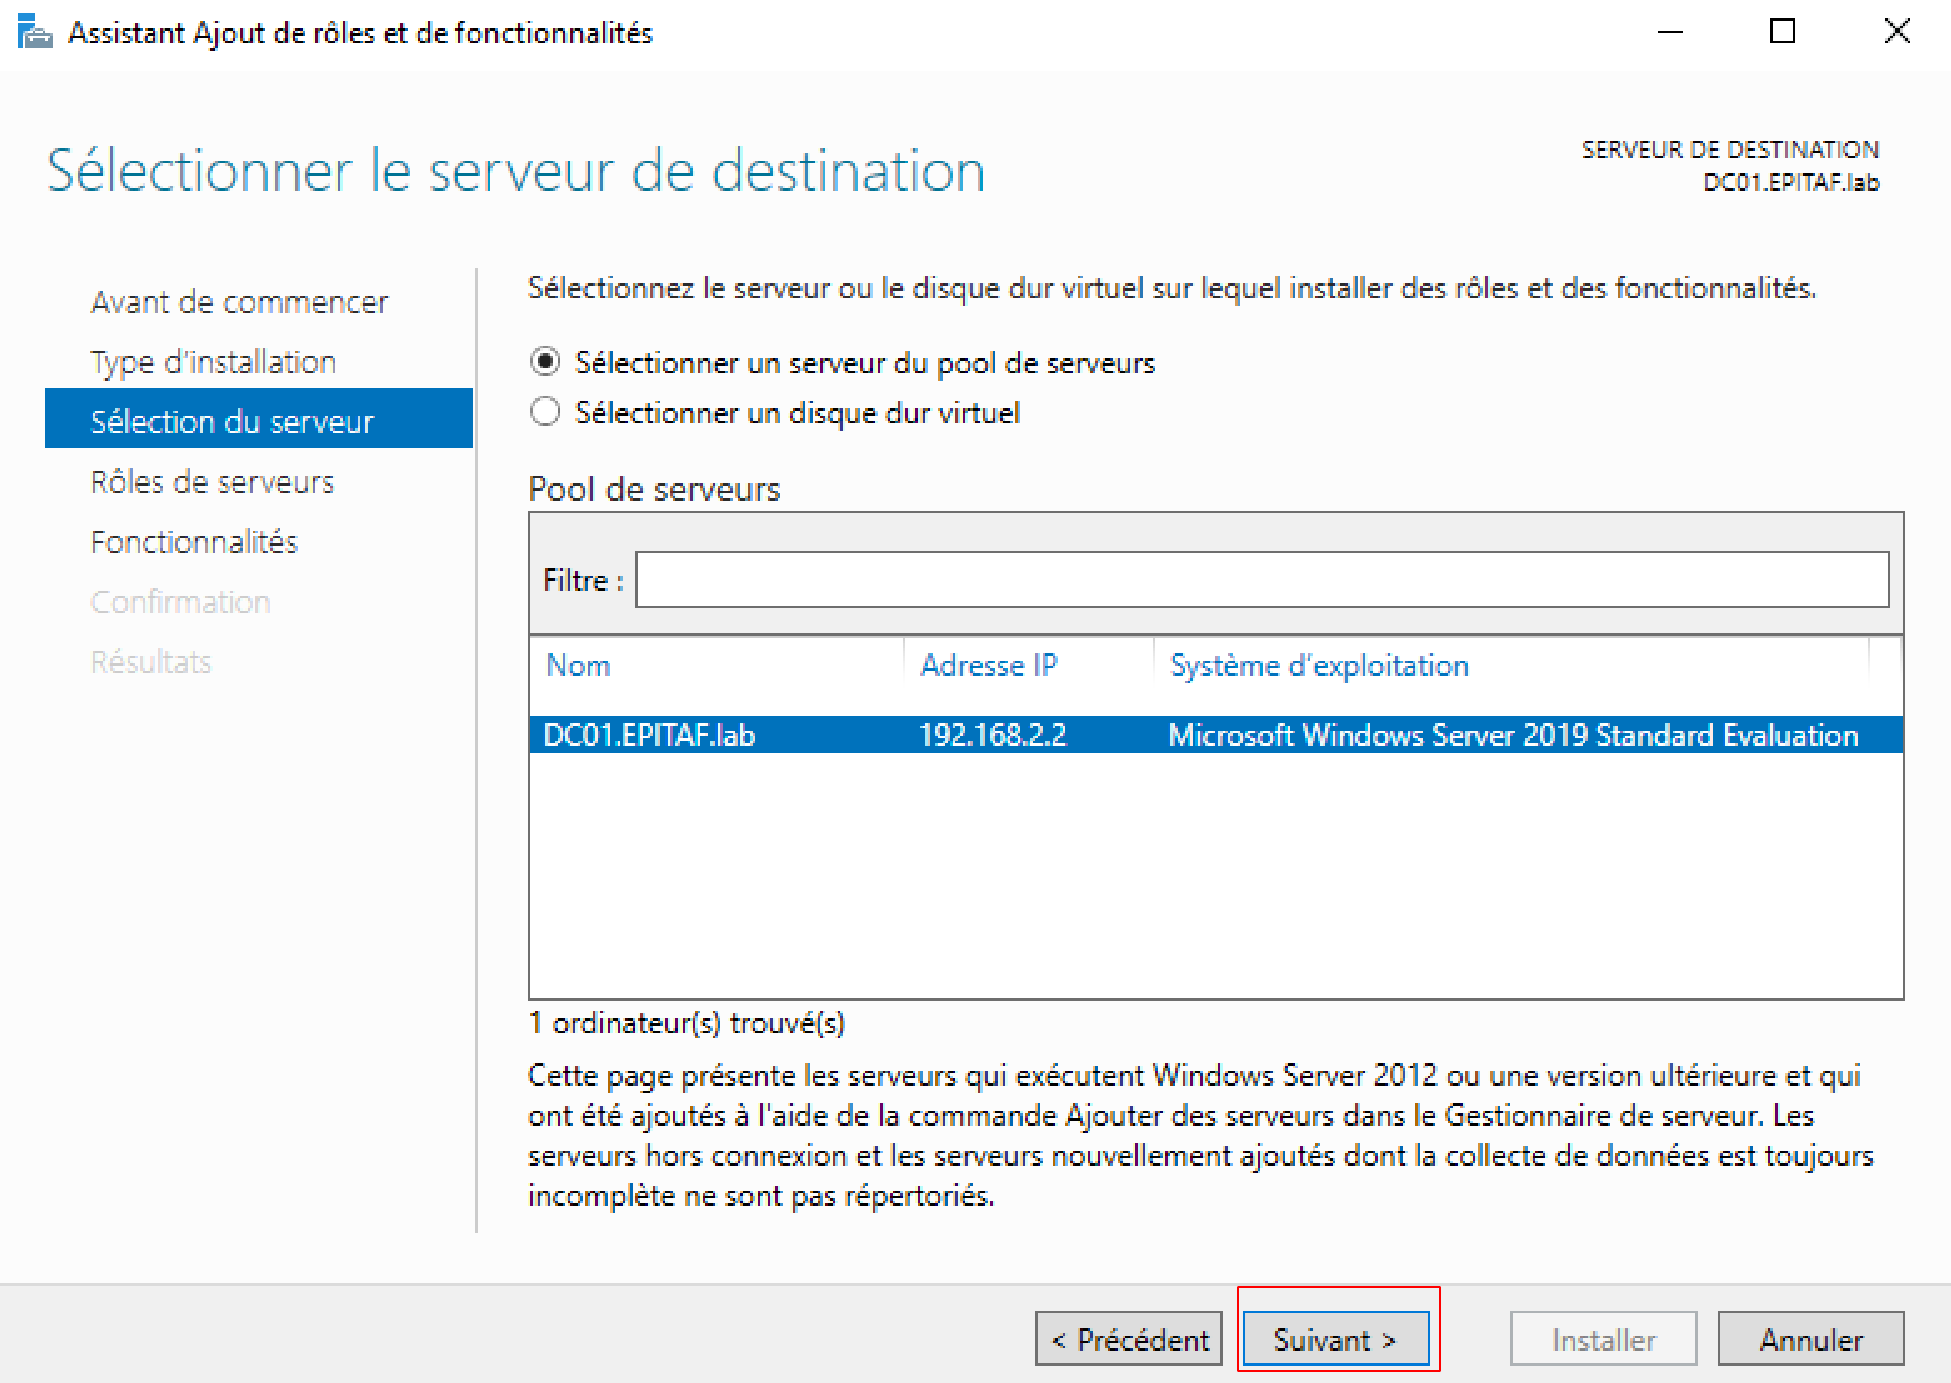
\includegraphics[scale=0.8]{WS_Screenshots/32.png}
		\label{Funcs_WinS/4}
	\end{center}
\end{figure}
\FloatBarrier 
    

\begin{figure}[h!]
	\begin{center}
		\caption{Ajout des rôles - Rôles et fonctionnalités de windows server}
		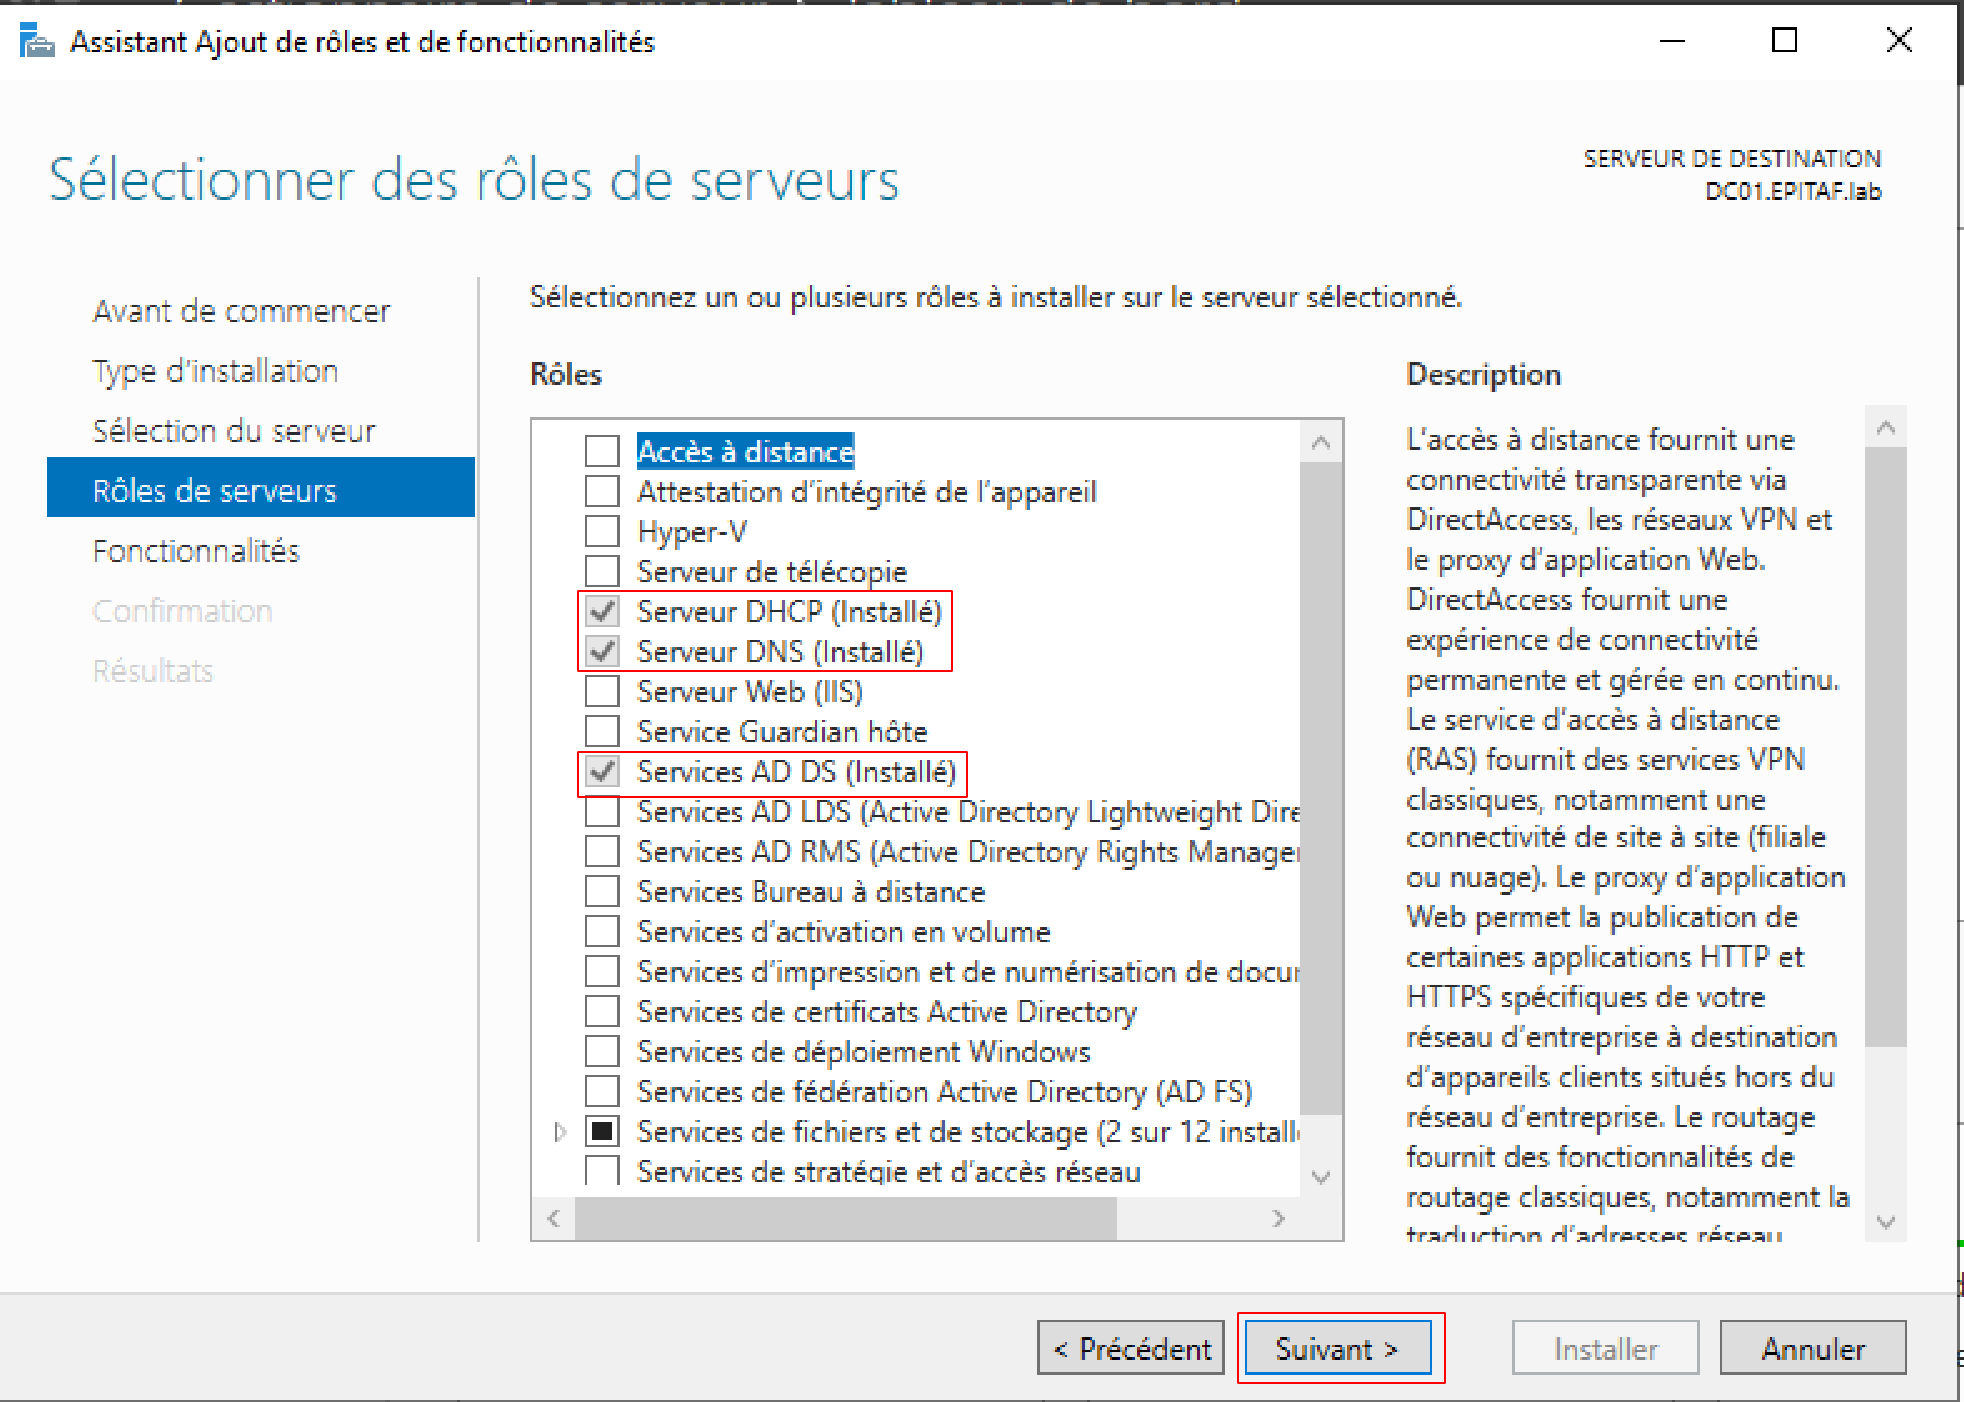
\includegraphics[scale=0.7]{WS_Screenshots/33.png}
		\label{Funcs_WinS/5}
	\end{center}
\end{figure}
\FloatBarrier 
    

\begin{figure}[h!]
	\begin{center}
		\caption{Sélection des fonctionnalités - Rôles et fonctionnalités de windows server}
		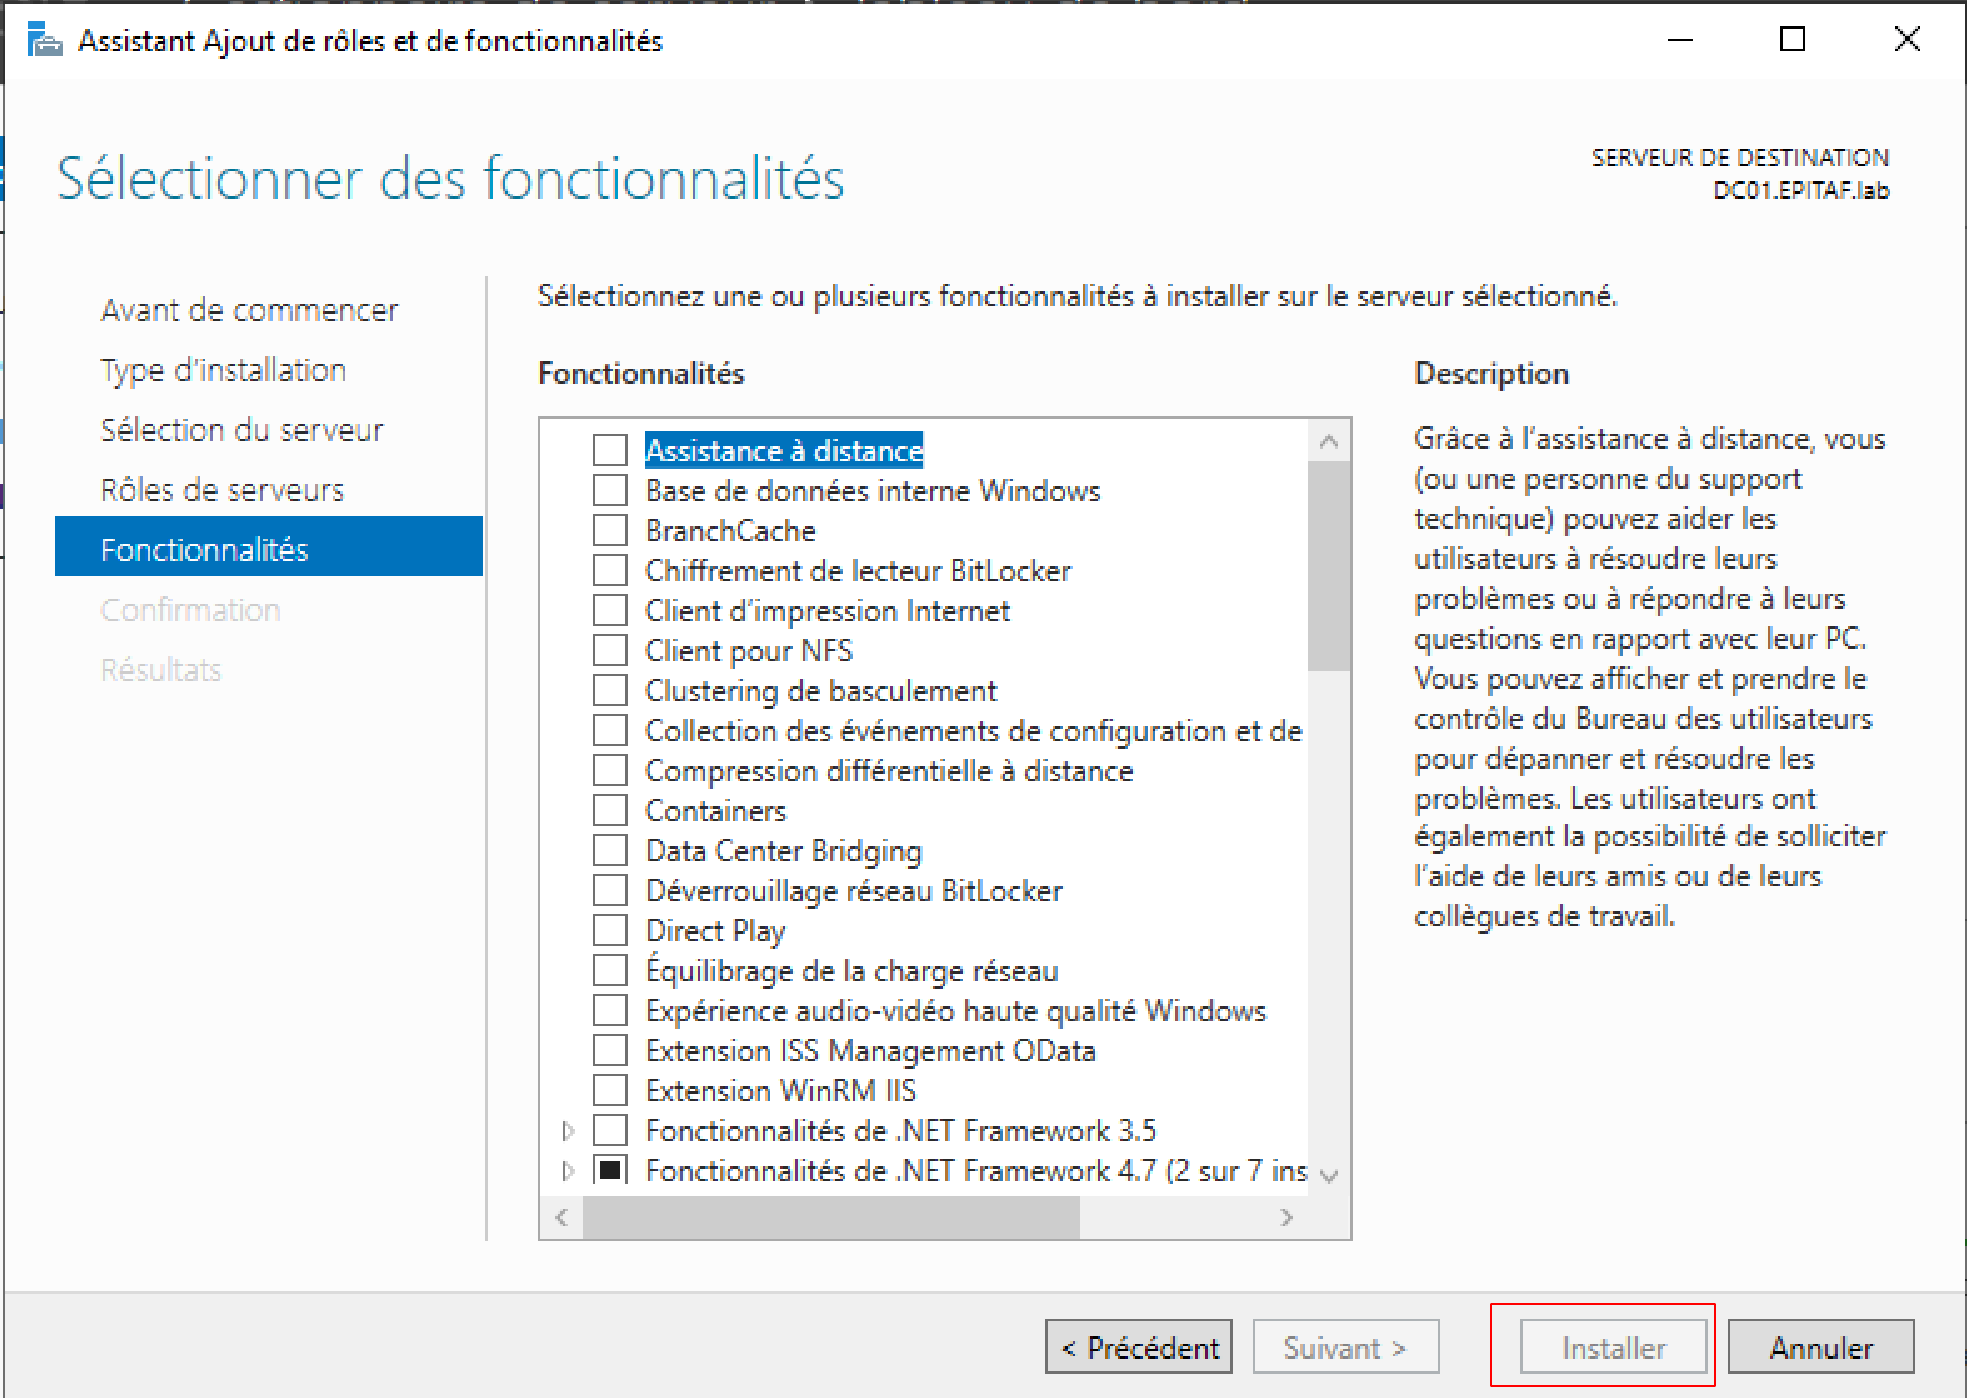
\includegraphics[scale=0.5]{WS_Screenshots/34.png}
		\label{Funcs_WinS/6}
	\end{center}
\end{figure}
\FloatBarrier 
    
\subsection{Gestion du DHCP}

\begin{itemize}
    \item Aller dans la section \textbf{DHCP} du gestionnaire de serveur. Cliquer droit sur la première entrée dans la table \textit{Serveurs}, et cliquer sur \textit{Gestionnaire DHCP} (figure \ref{Funcs_WinS/7});
    \item Cliquer sur le nom du serveur, puis aller dans \textit{Autres actions}. Cliquer sur autoriser dans le menu obtenu (figure \ref{Funcs_WinS/8}).
\end{itemize}

\begin{figure}[h!]
	\begin{center}
		\caption{Accès au gestionnaire DHCP de windows server}
		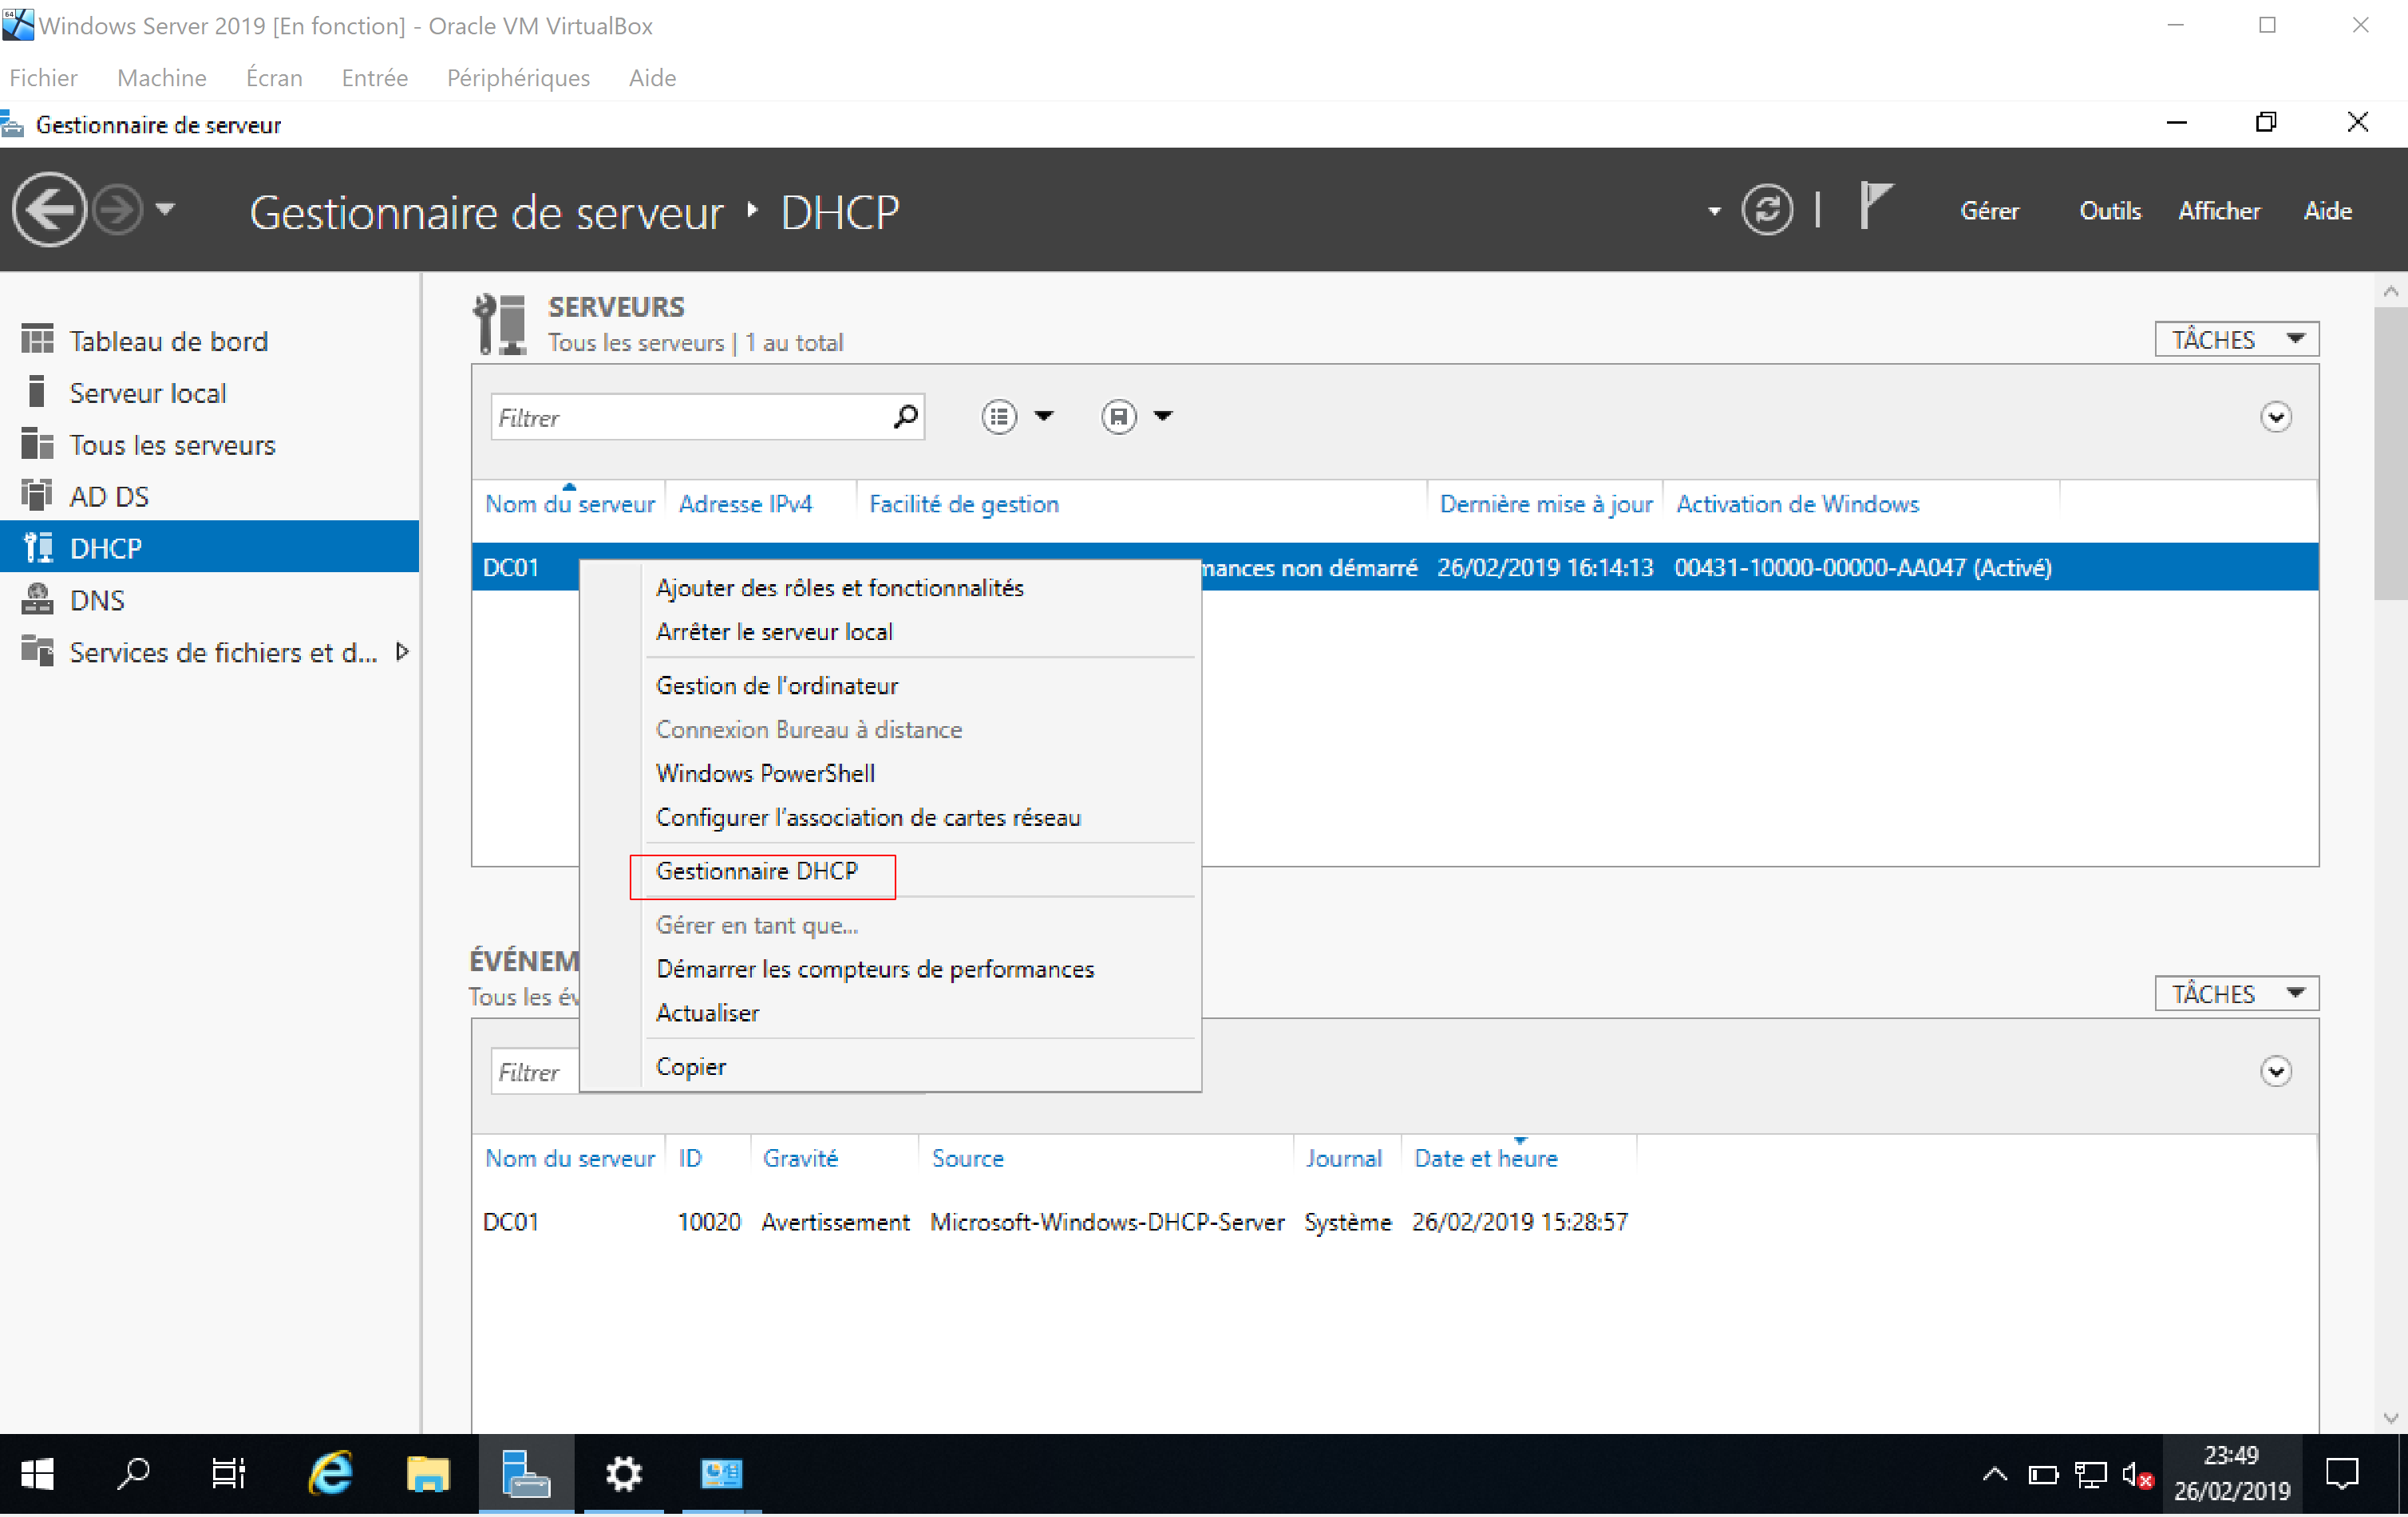
\includegraphics[scale=0.5]{WS_Screenshots/35.png}
		\label{Funcs_WinS/7}
	\end{center}
\end{figure}
\FloatBarrier 
    

\begin{figure}[h!]
	\begin{center}
		\caption{Autorisation - Gestionnaire DHCP de windows server}
		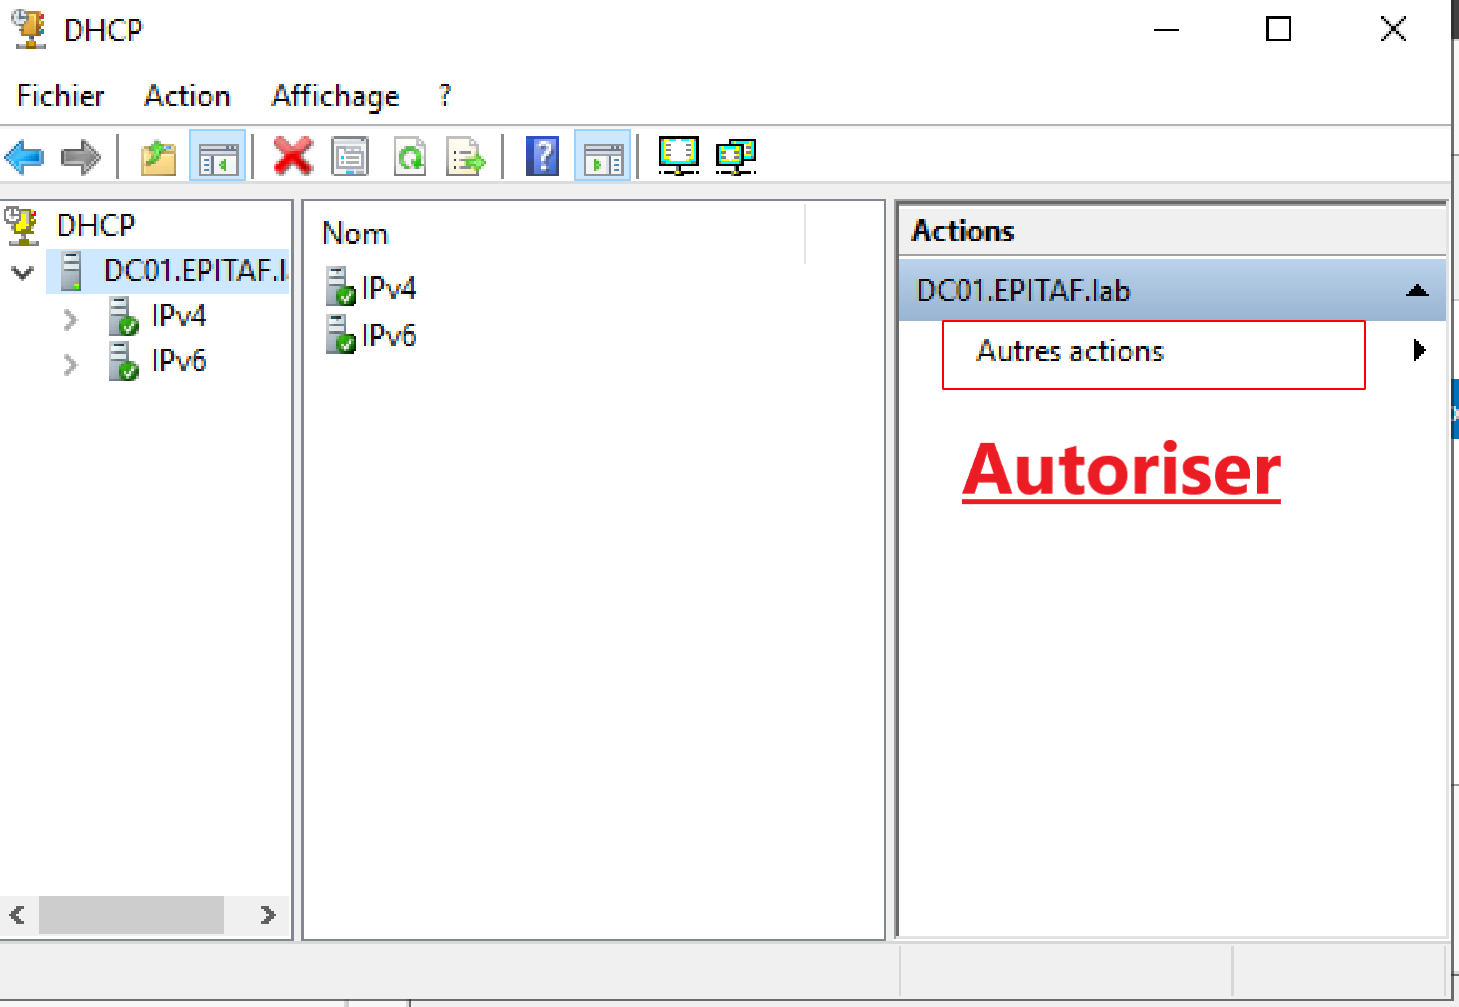
\includegraphics[scale=0.3]{WS_Screenshots/36.png}
		\label{Funcs_WinS/8}
	\end{center}
\end{figure}
\FloatBarrier 
    
\subsubsection{Ajout d'une étendue DHCP}

\begin{itemize}
    \item Dans la même fenêtre que précédemment, cliquer droit sur \texttt{IPv4}, puis sélectionner \textit{Nouvelle étendue...} (figure \ref{Funcs_WinS/9});
    \item Cliquer sur \textit{Suivant} dans la fenêtre de l'assistant de nouvelle étendue (figure \ref{Funcs_WinS/10});
    \item Renseigner le nom \textbf{EPITAF} dans le champ \textit{Nom}. Cliquer sur \textit{Suivant} (figure \ref{Funcs_WinS/11});
    \item Rentrer les valeurs suivantes dans les quatre champs :
    \begin{itemize}
        \item \texttt{Adresse IP de début} : 192.168.2.10;
        \item \texttt{Adresse IP de fin} : 192.168.2.20;
        \item \texttt{Longueur} : 24;
        \item \texttt{Masque de sous-réseau} : 255.255.255.0.
    \end{itemize}
    Cliquer sur \textit{Suivant} (figure \ref{Funcs_WinS/12});
    \item Cliquer sur \textit{Suivant} (figure \ref{Funcs_WinS/13});
    \item Cliquer sur \textit{Suivant} (figure \ref{Funcs_WinS/14});
    \item Sélectionner l'option "\textit{Oui, je veux configurer ces options maintenant}", puis cliquer sur \textit{Suivant} (figure \ref{Funcs_WinS/15});
    \item Cliquer sur \textit{Suivant} (figure \ref{Funcs_WinS/16});
    \item Renseigner le nom \texttt{EPITAF.lab} dans le champ \textit{Domaine parent}. Ajouter l'adresse IP \textit{192.168.2.2} dans le champ \textit{Adresse IP}. Cliquer sur \textit{Suivant} (figure \ref{Funcs_WinS/17});
    \item Cliquer sur \textit{Suivnat} (figure \ref{Funcs_WinS/18});
    \item Sélectionner l'option "\textit{Oui, je veux activer cette étendue maintenant}", puis cliquer sur \textit{Suivant} (figure \ref{Funcs_WinS/19});
    \item Cliquer sur \textit{Terminer} à la fin de l'Assistant de Nouvelle étendue de windows server (figure \ref{Funcs_WinS/20}).
\end{itemize}

\begin{figure}[h!]
	\begin{center}
		\caption{Nouvelle étendue - Gestionnaire DHCP de windows server}
		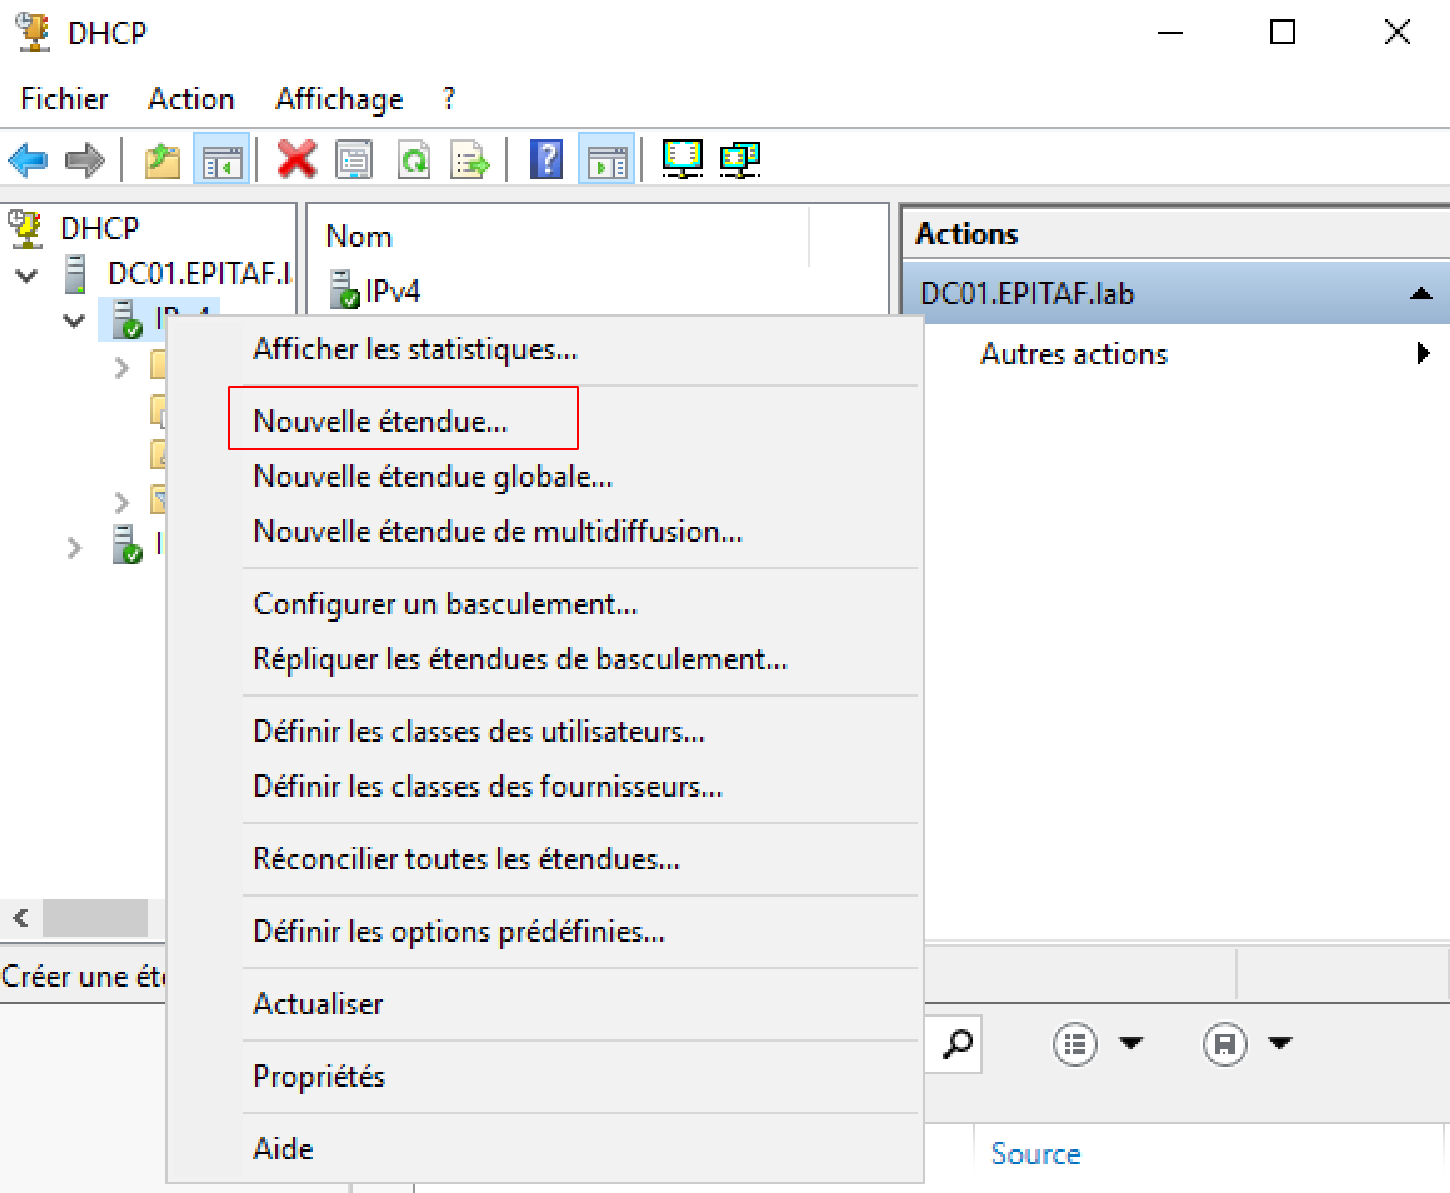
\includegraphics[scale=0.7]{WS_Screenshots/37.png}
		\label{Funcs_WinS/9}
	\end{center}
\end{figure}
\FloatBarrier 
    

\begin{figure}[h!]
	\begin{center}
		\caption{Assistant de Nouvelle étendue - Gestionnaire DHCP de windows server}
		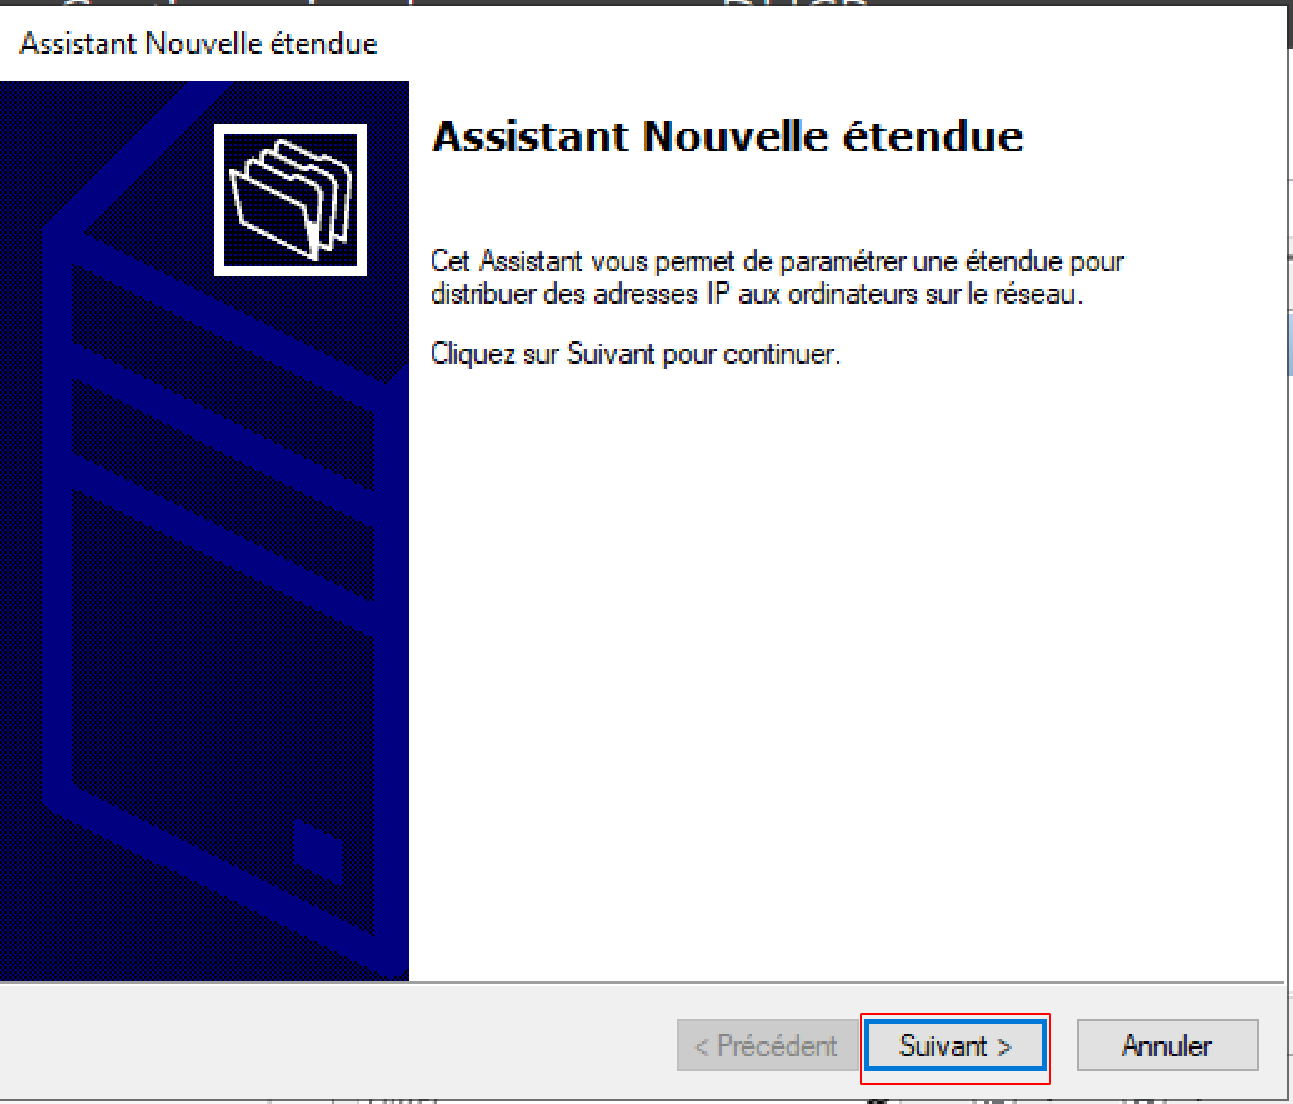
\includegraphics[scale=0.7]{WS_Screenshots/38.png}
		\label{Funcs_WinS/10}
	\end{center}
\end{figure}
\FloatBarrier 
    
\begin{figure}[h!]
	\begin{center}
		\caption{Attribution du nom - Assistant de Nouvelle étendue de windows server}
		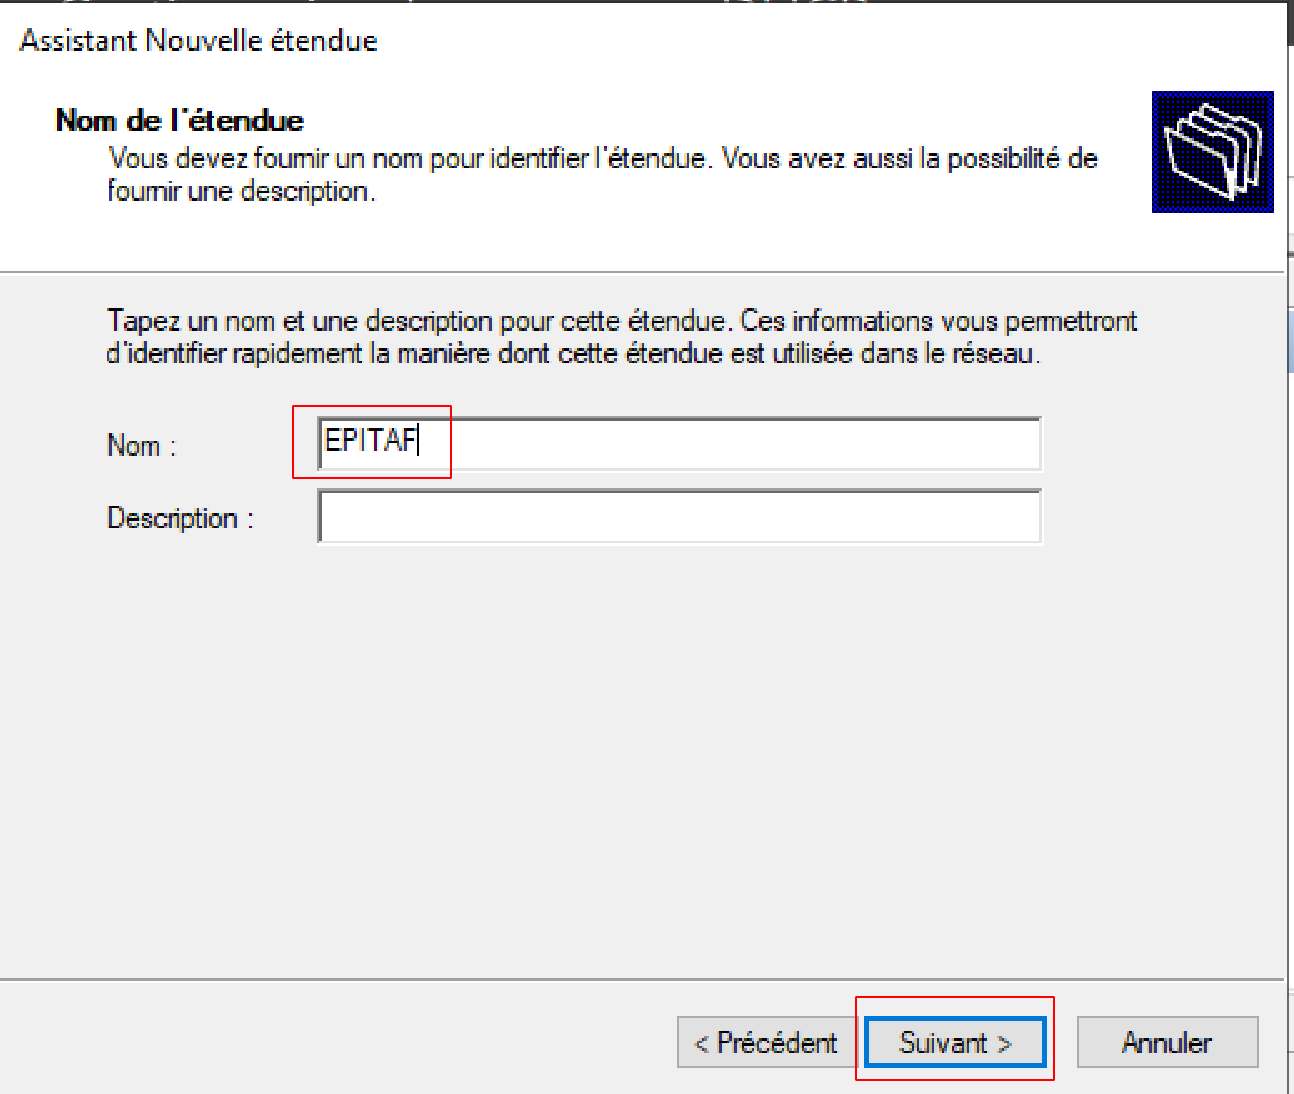
\includegraphics[scale=0.7]{WS_Screenshots/39.png}
		\label{Funcs_WinS/11}
	\end{center}
\end{figure}
\FloatBarrier 
    

\begin{figure}[h!]
	\begin{center}
		\caption{Attribution de la plage d'adresses - Assistant de Nouvelle étendue de windows server}
		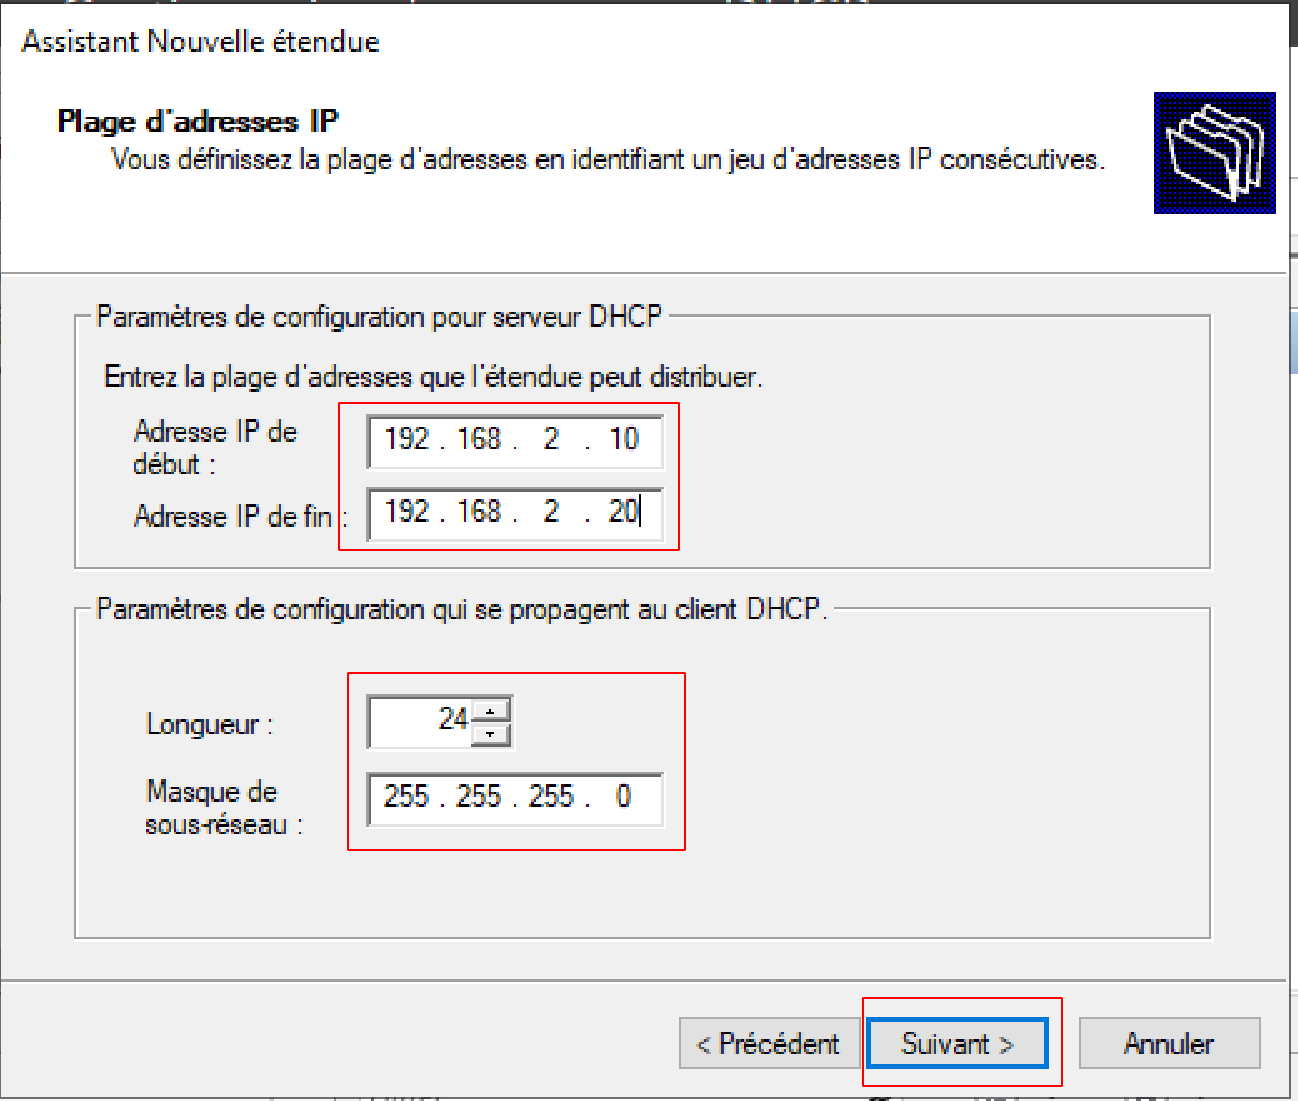
\includegraphics[scale=0.7]{WS_Screenshots/40.png}
		\label{Funcs_WinS/12}
	\end{center}
\end{figure}
\FloatBarrier 
    

\begin{figure}[h!]
	\begin{center}
		\caption{Menu d'ajout d'exclusions et retards - Assistant de Nouvelle étendue de windows server}
		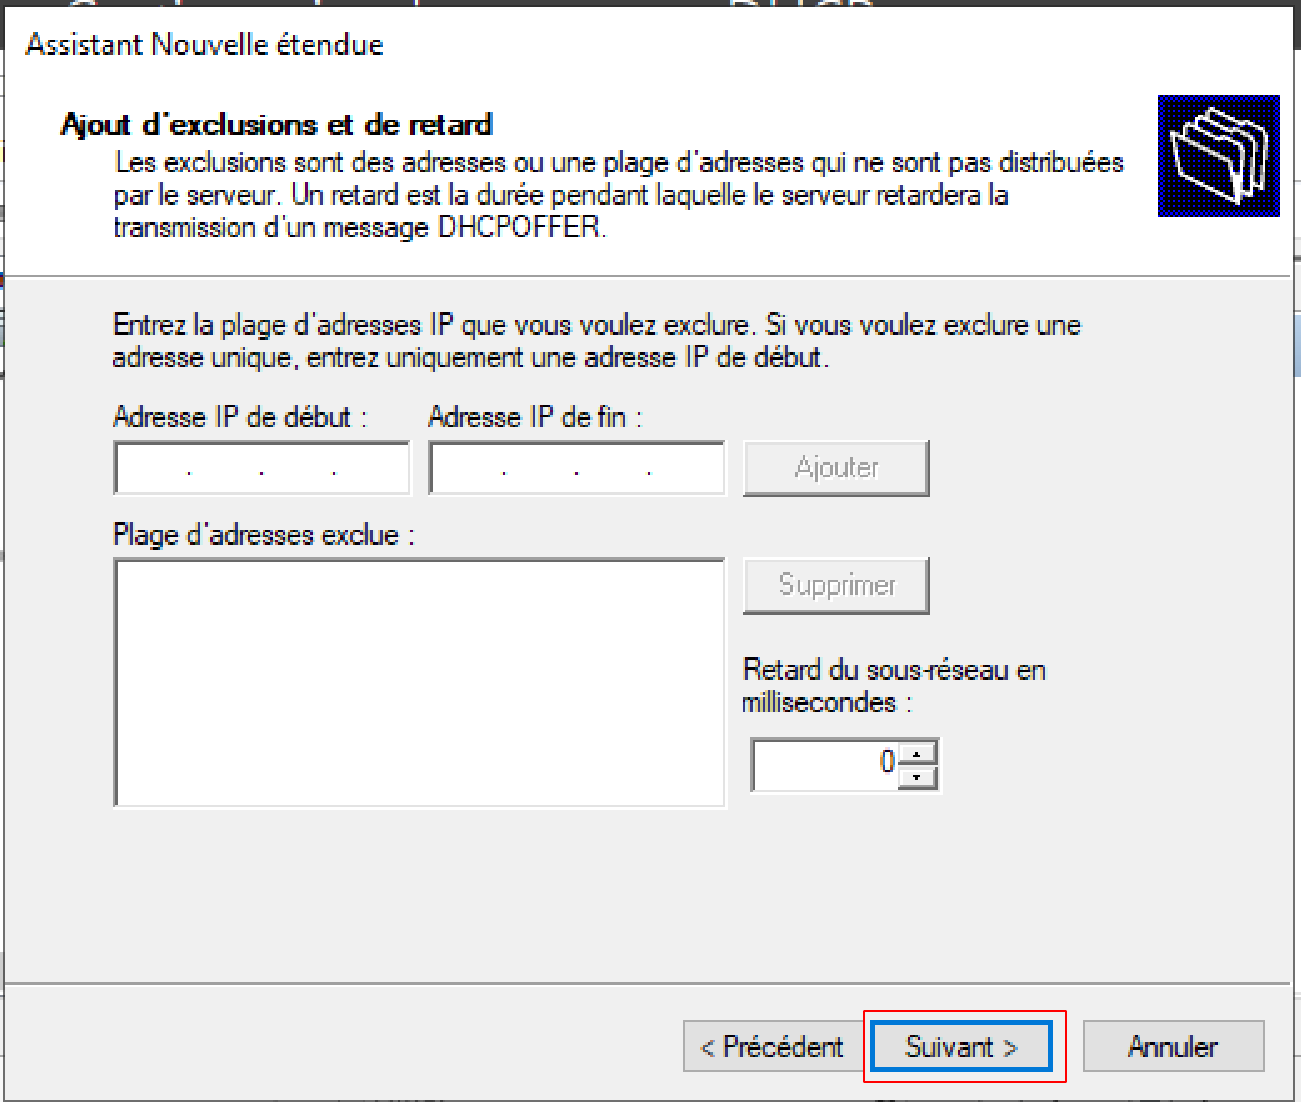
\includegraphics[scale=0.7]{WS_Screenshots/41.png}
		\label{Funcs_WinS/13}
	\end{center}
\end{figure}
\FloatBarrier 
    

\begin{figure}[h!]
	\begin{center}
		\caption{Durée du bail - Assistant de Nouvelle étendue de windows server}
		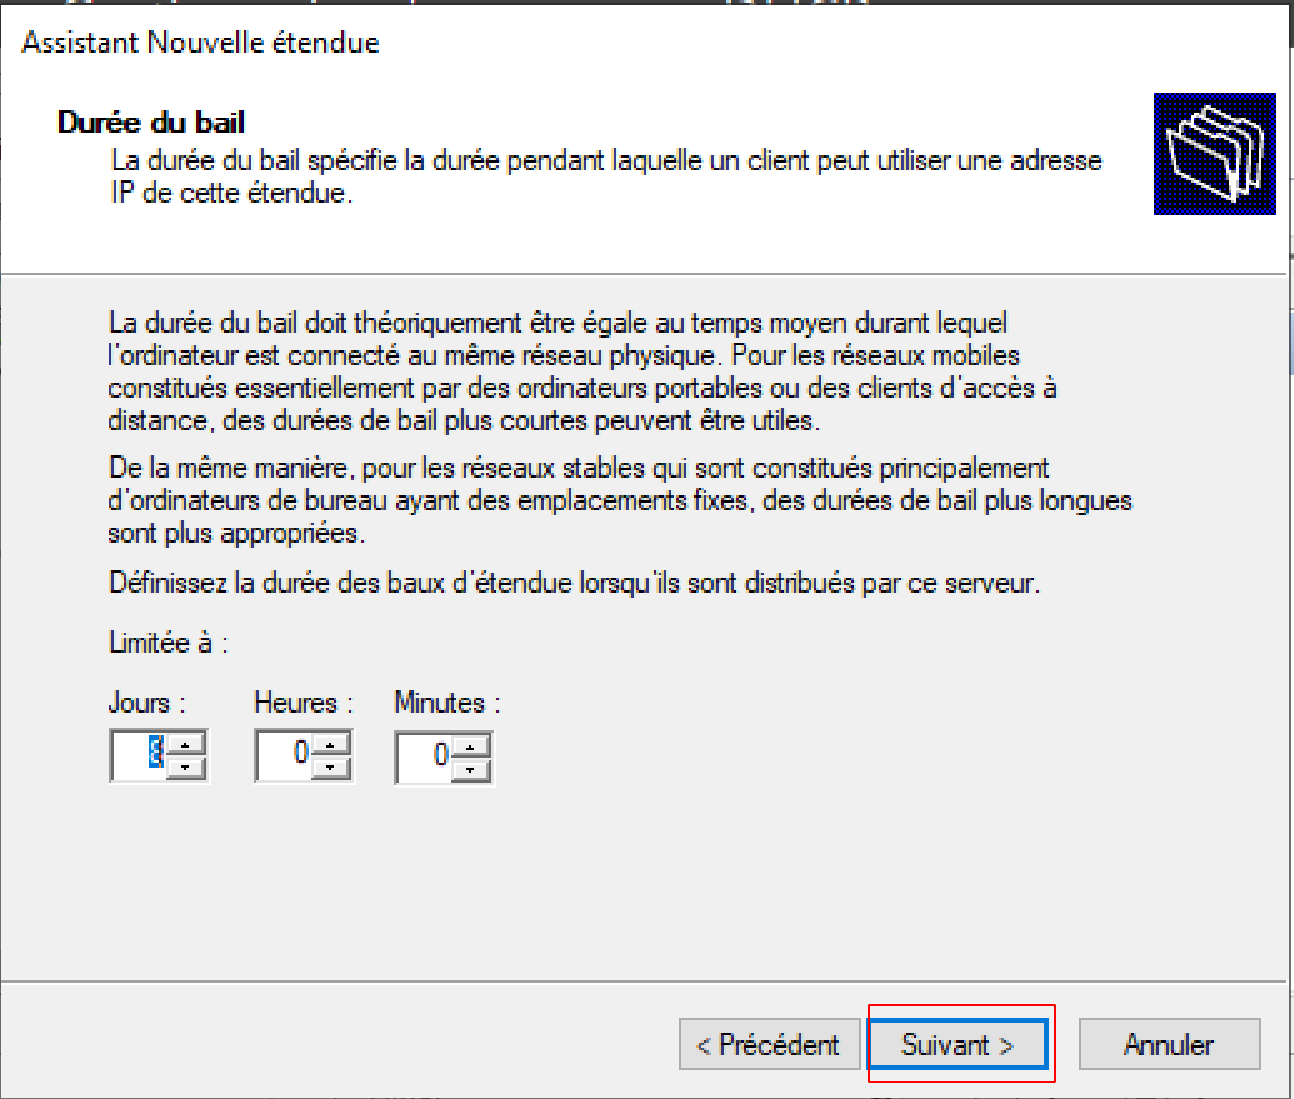
\includegraphics[scale=0.7]{WS_Screenshots/42.png}
		\label{Funcs_WinS/14}
	\end{center}
\end{figure}
\FloatBarrier 
    

\begin{figure}[h!]
	\begin{center}
		\caption{Configuration des paramètres DHCP - Assistant de Nouvelle étendue de windows server}
		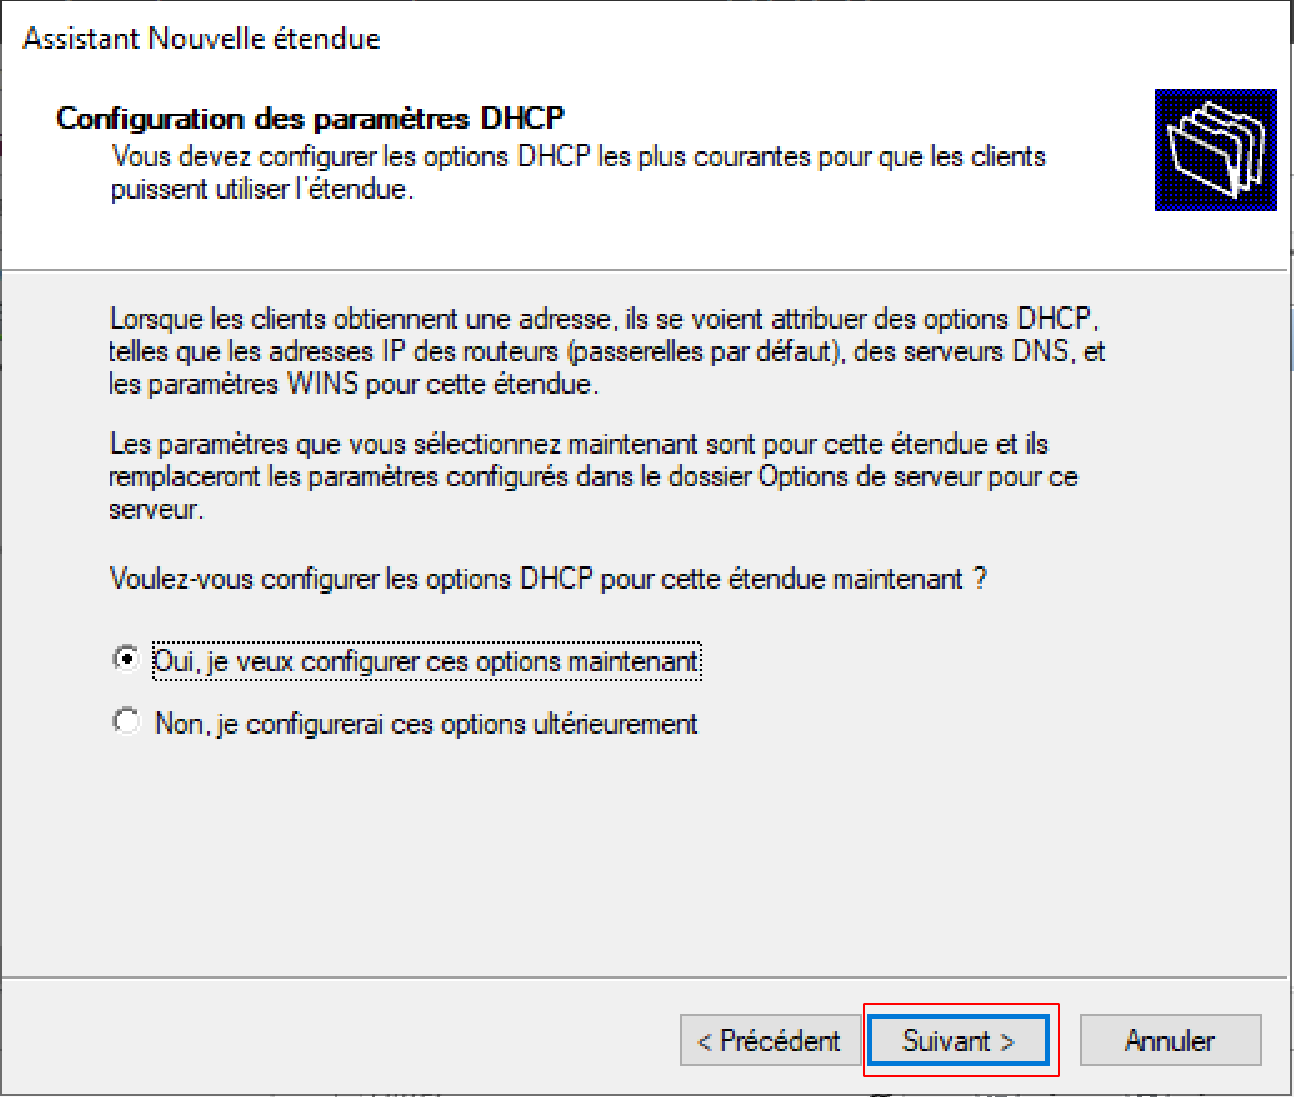
\includegraphics[scale=0.7]{WS_Screenshots/43.png}
		\label{Funcs_WinS/15}
	\end{center}
\end{figure}
\FloatBarrier 
    

\begin{figure}[h!]
	\begin{center}
		\caption{Routeur - Assistant de Nouvelle étendue de windows server}
		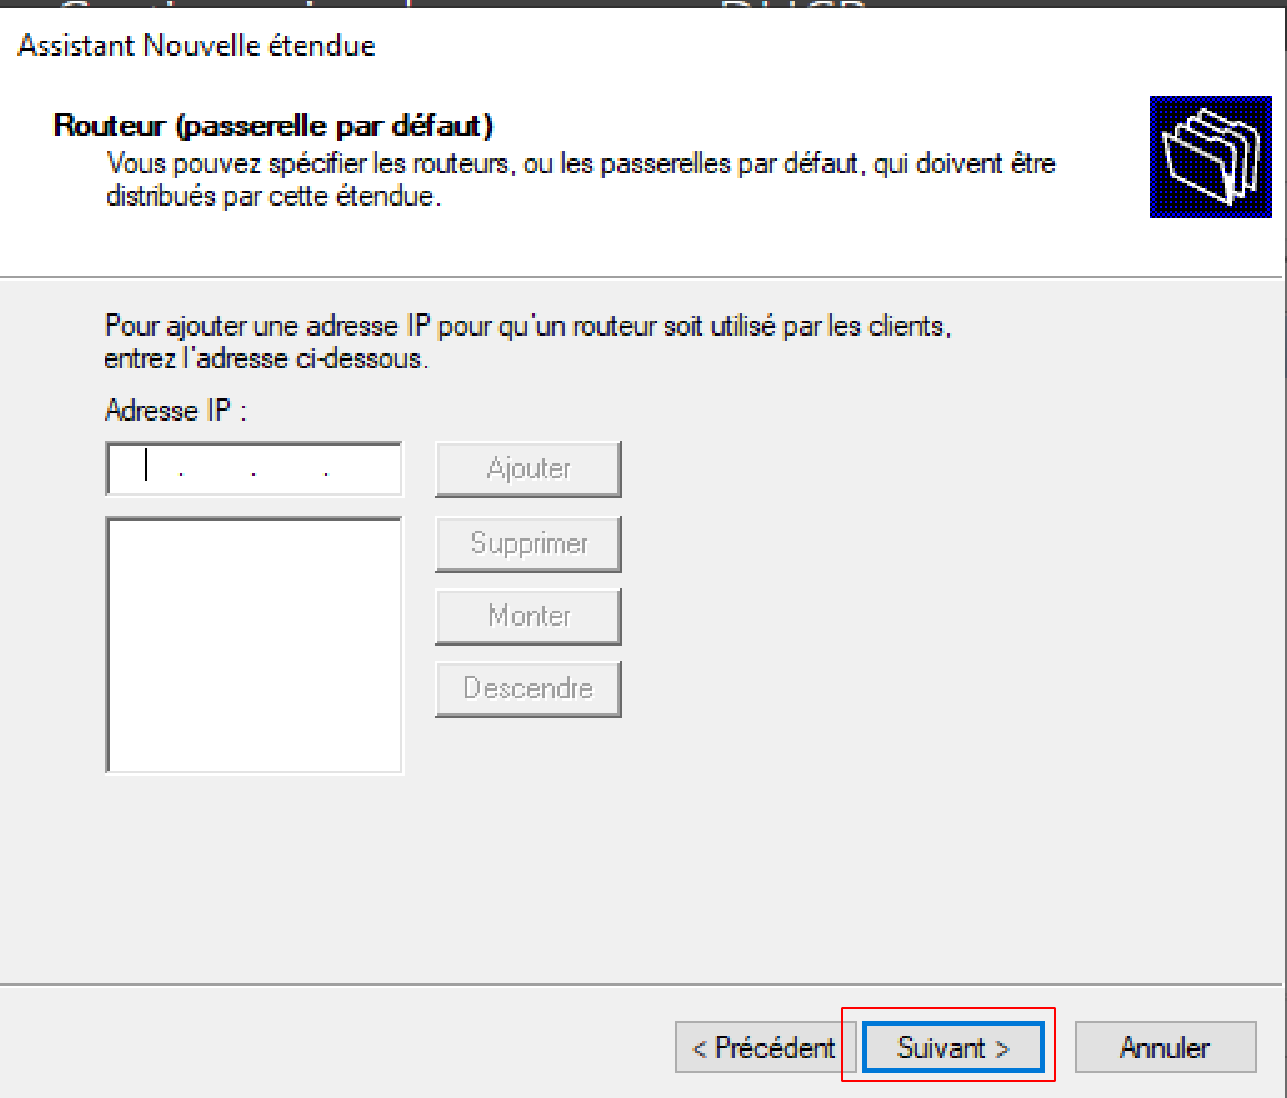
\includegraphics[scale=0.7]{WS_Screenshots/44.png}
		\label{Funcs_WinS/16}
	\end{center}
\end{figure}
\FloatBarrier 
    

\begin{figure}[h!]
	\begin{center}
		\caption{Nom de domaine et serveurs DNS - Assistant de Nouvelle étendue de windows server}
		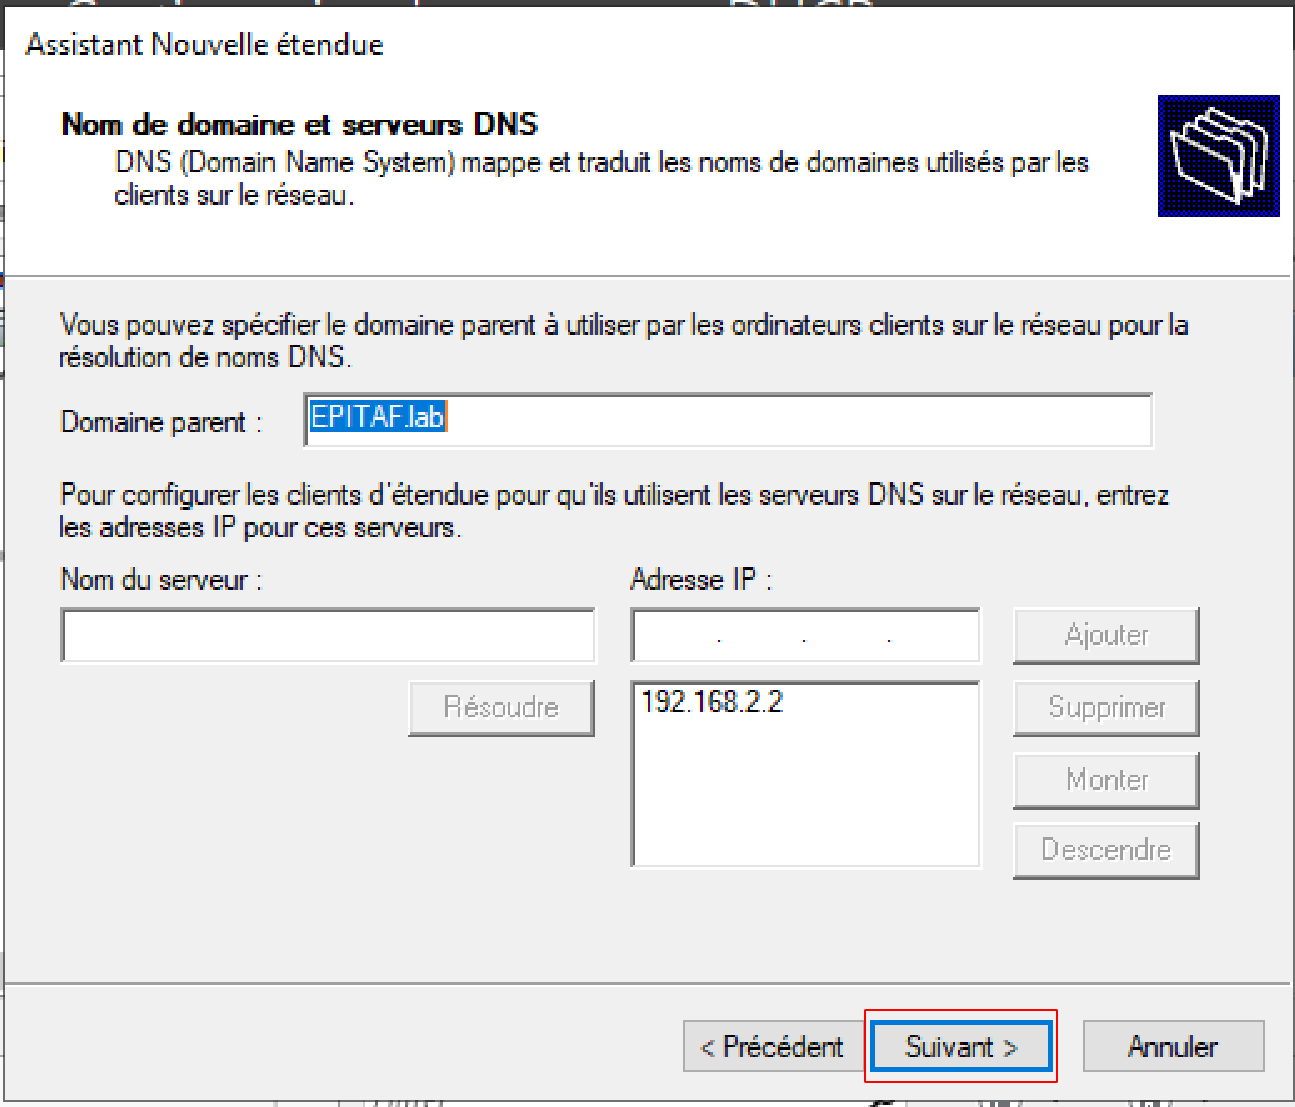
\includegraphics[scale=0.7]{WS_Screenshots/45.png}
		\label{Funcs_WinS/17}
	\end{center}
\end{figure}
\FloatBarrier 
    

\begin{figure}[h!]
	\begin{center}
		\caption{Serveurs WINS - Assistant de Nouvelle étendue de windows server}
		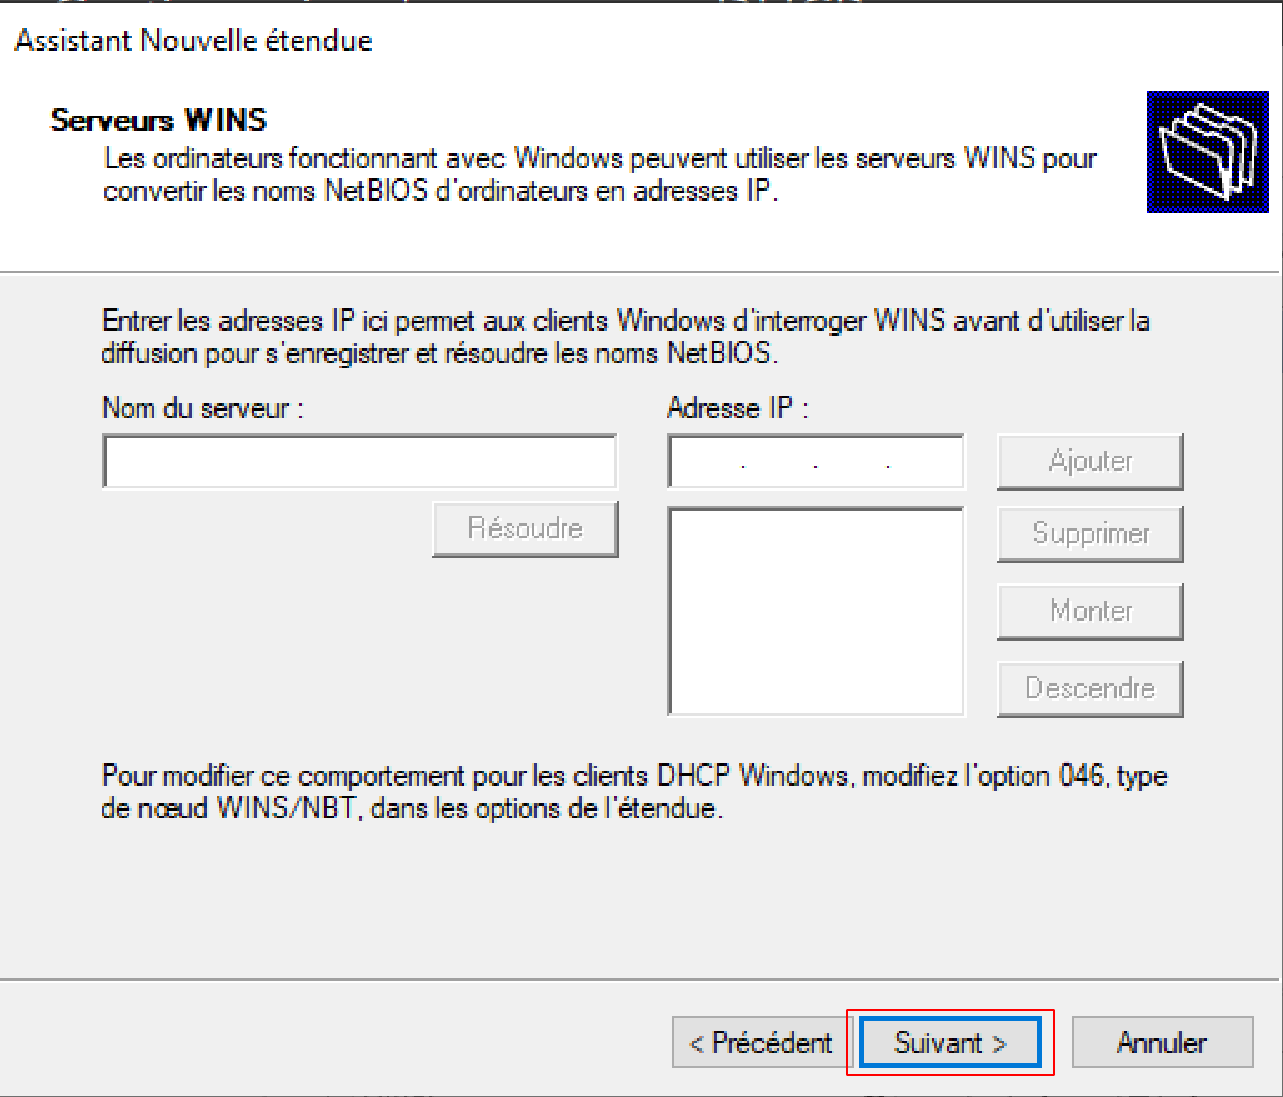
\includegraphics[scale=0.7]{WS_Screenshots/46.png}
		\label{Funcs_WinS/18}
	\end{center}
\end{figure}
\FloatBarrier 
    

\begin{figure}[h!]
	\begin{center}
		\caption{Activation de l'étendue - Assistant de Nouvelle étendue de windows server}
		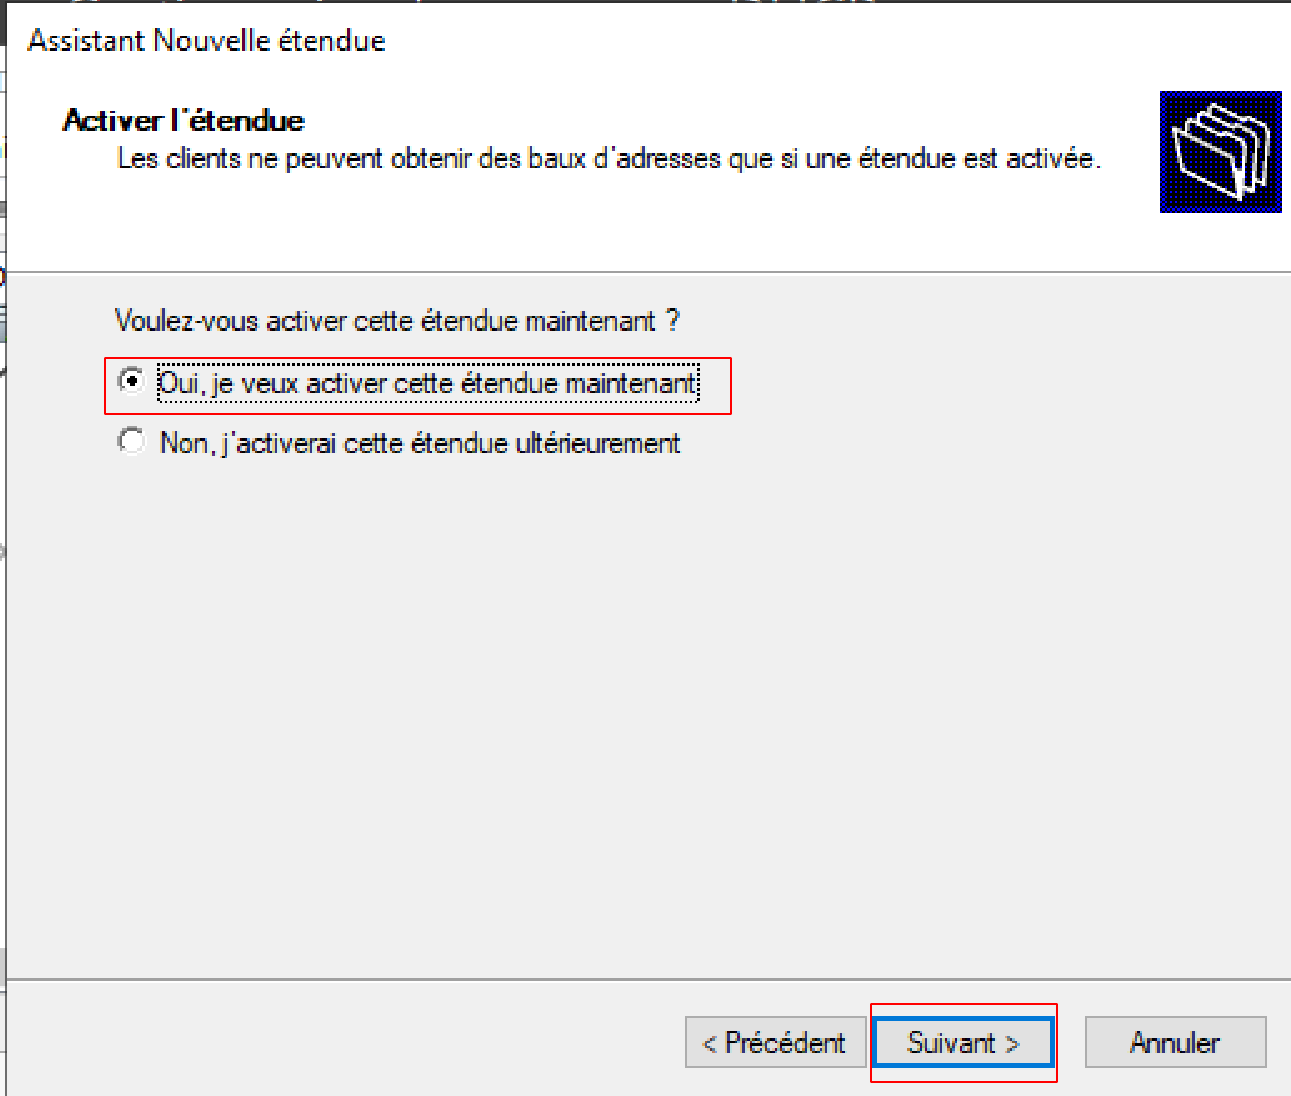
\includegraphics[scale=0.8]{WS_Screenshots/47.png}
		\label{Funcs_WinS/19}
	\end{center}
\end{figure}
\FloatBarrier 
    

\begin{figure}[h!]
	\begin{center}
		\caption{Fin de l'Assistant de Nouvelle étendue de windows server}
		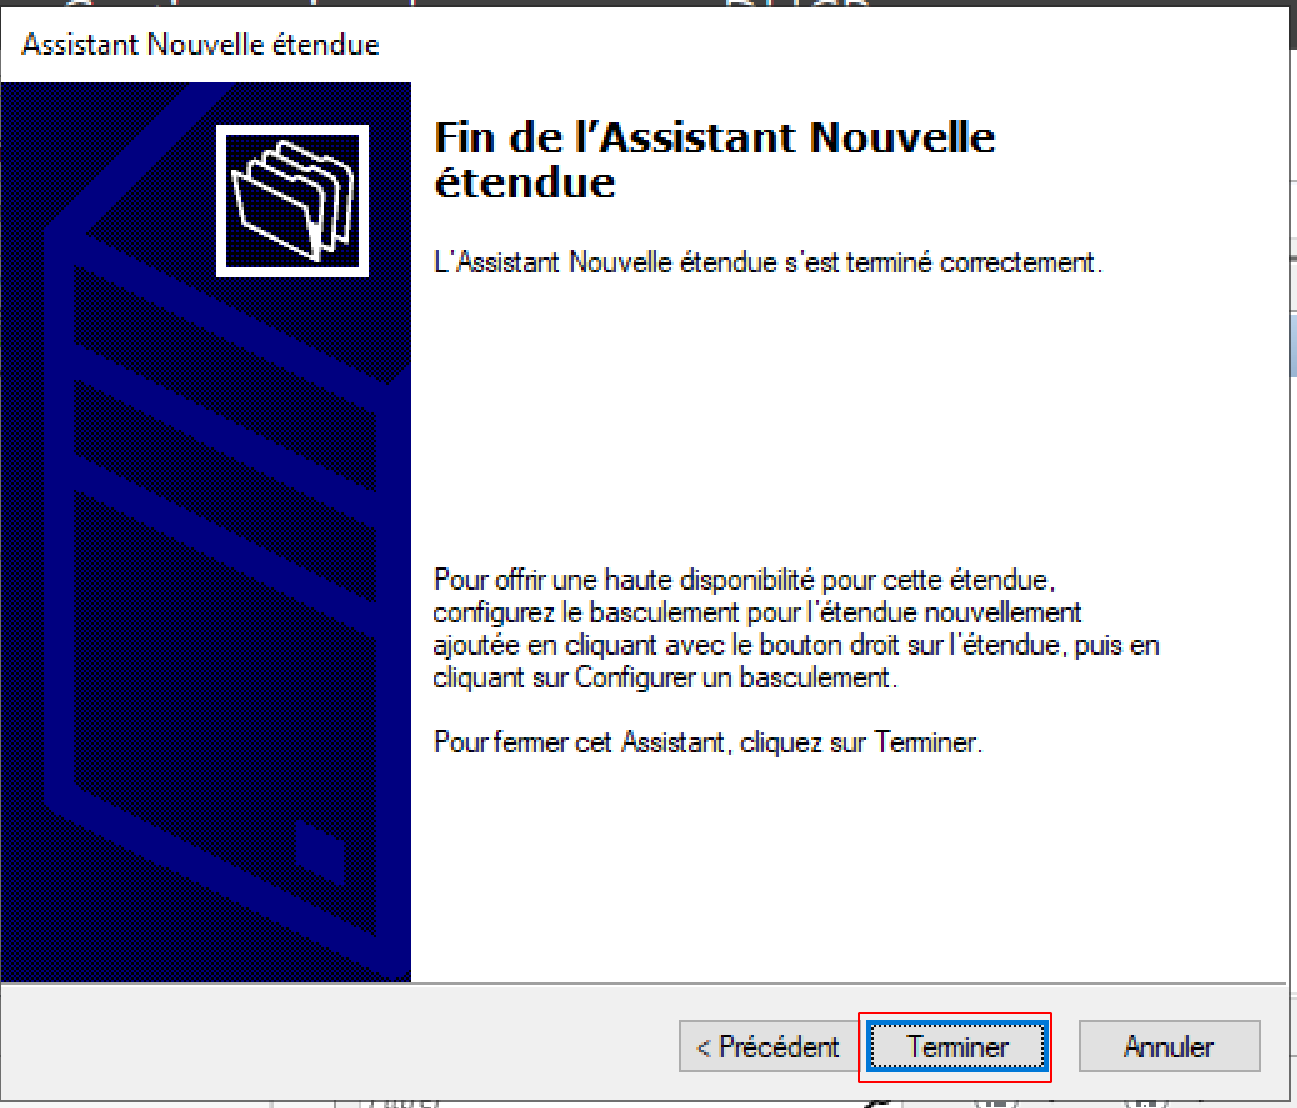
\includegraphics[scale=0.8]{WS_Screenshots/48.png}
		\label{Funcs_WinS/20}
	\end{center}
\end{figure}
\FloatBarrier 
    
\subsection{Configuration du DNS}

\begin{itemize}
    \item Aller dans la section \textbf{DNS} du gestionnaire de serveur. Cliquer droit sur la première entrée dans la table \textit{Serveurs}, et cliquer sur \textit{Gestionnaire DNS} (figure \ref{Funcs_WinS/21});
    \item Dans la section \texttt{Redirecteurs}, cliquer sur \textit{Modifier} (figure \ref{Funcs_WinS/22});
    \item Ajouter l'adresse IP \texttt{8.8.8.8}, puis cliquer sur \textit{OK} (figure \ref{Funcs_WinS/23});
    \item Cliquer sur \textit{OK} (figure \ref{Funcs_WinS/24}).
\end{itemize}

\begin{figure}[h!]
	\begin{center}
		\caption{Accès au gestionnaire DNS de windows server}
		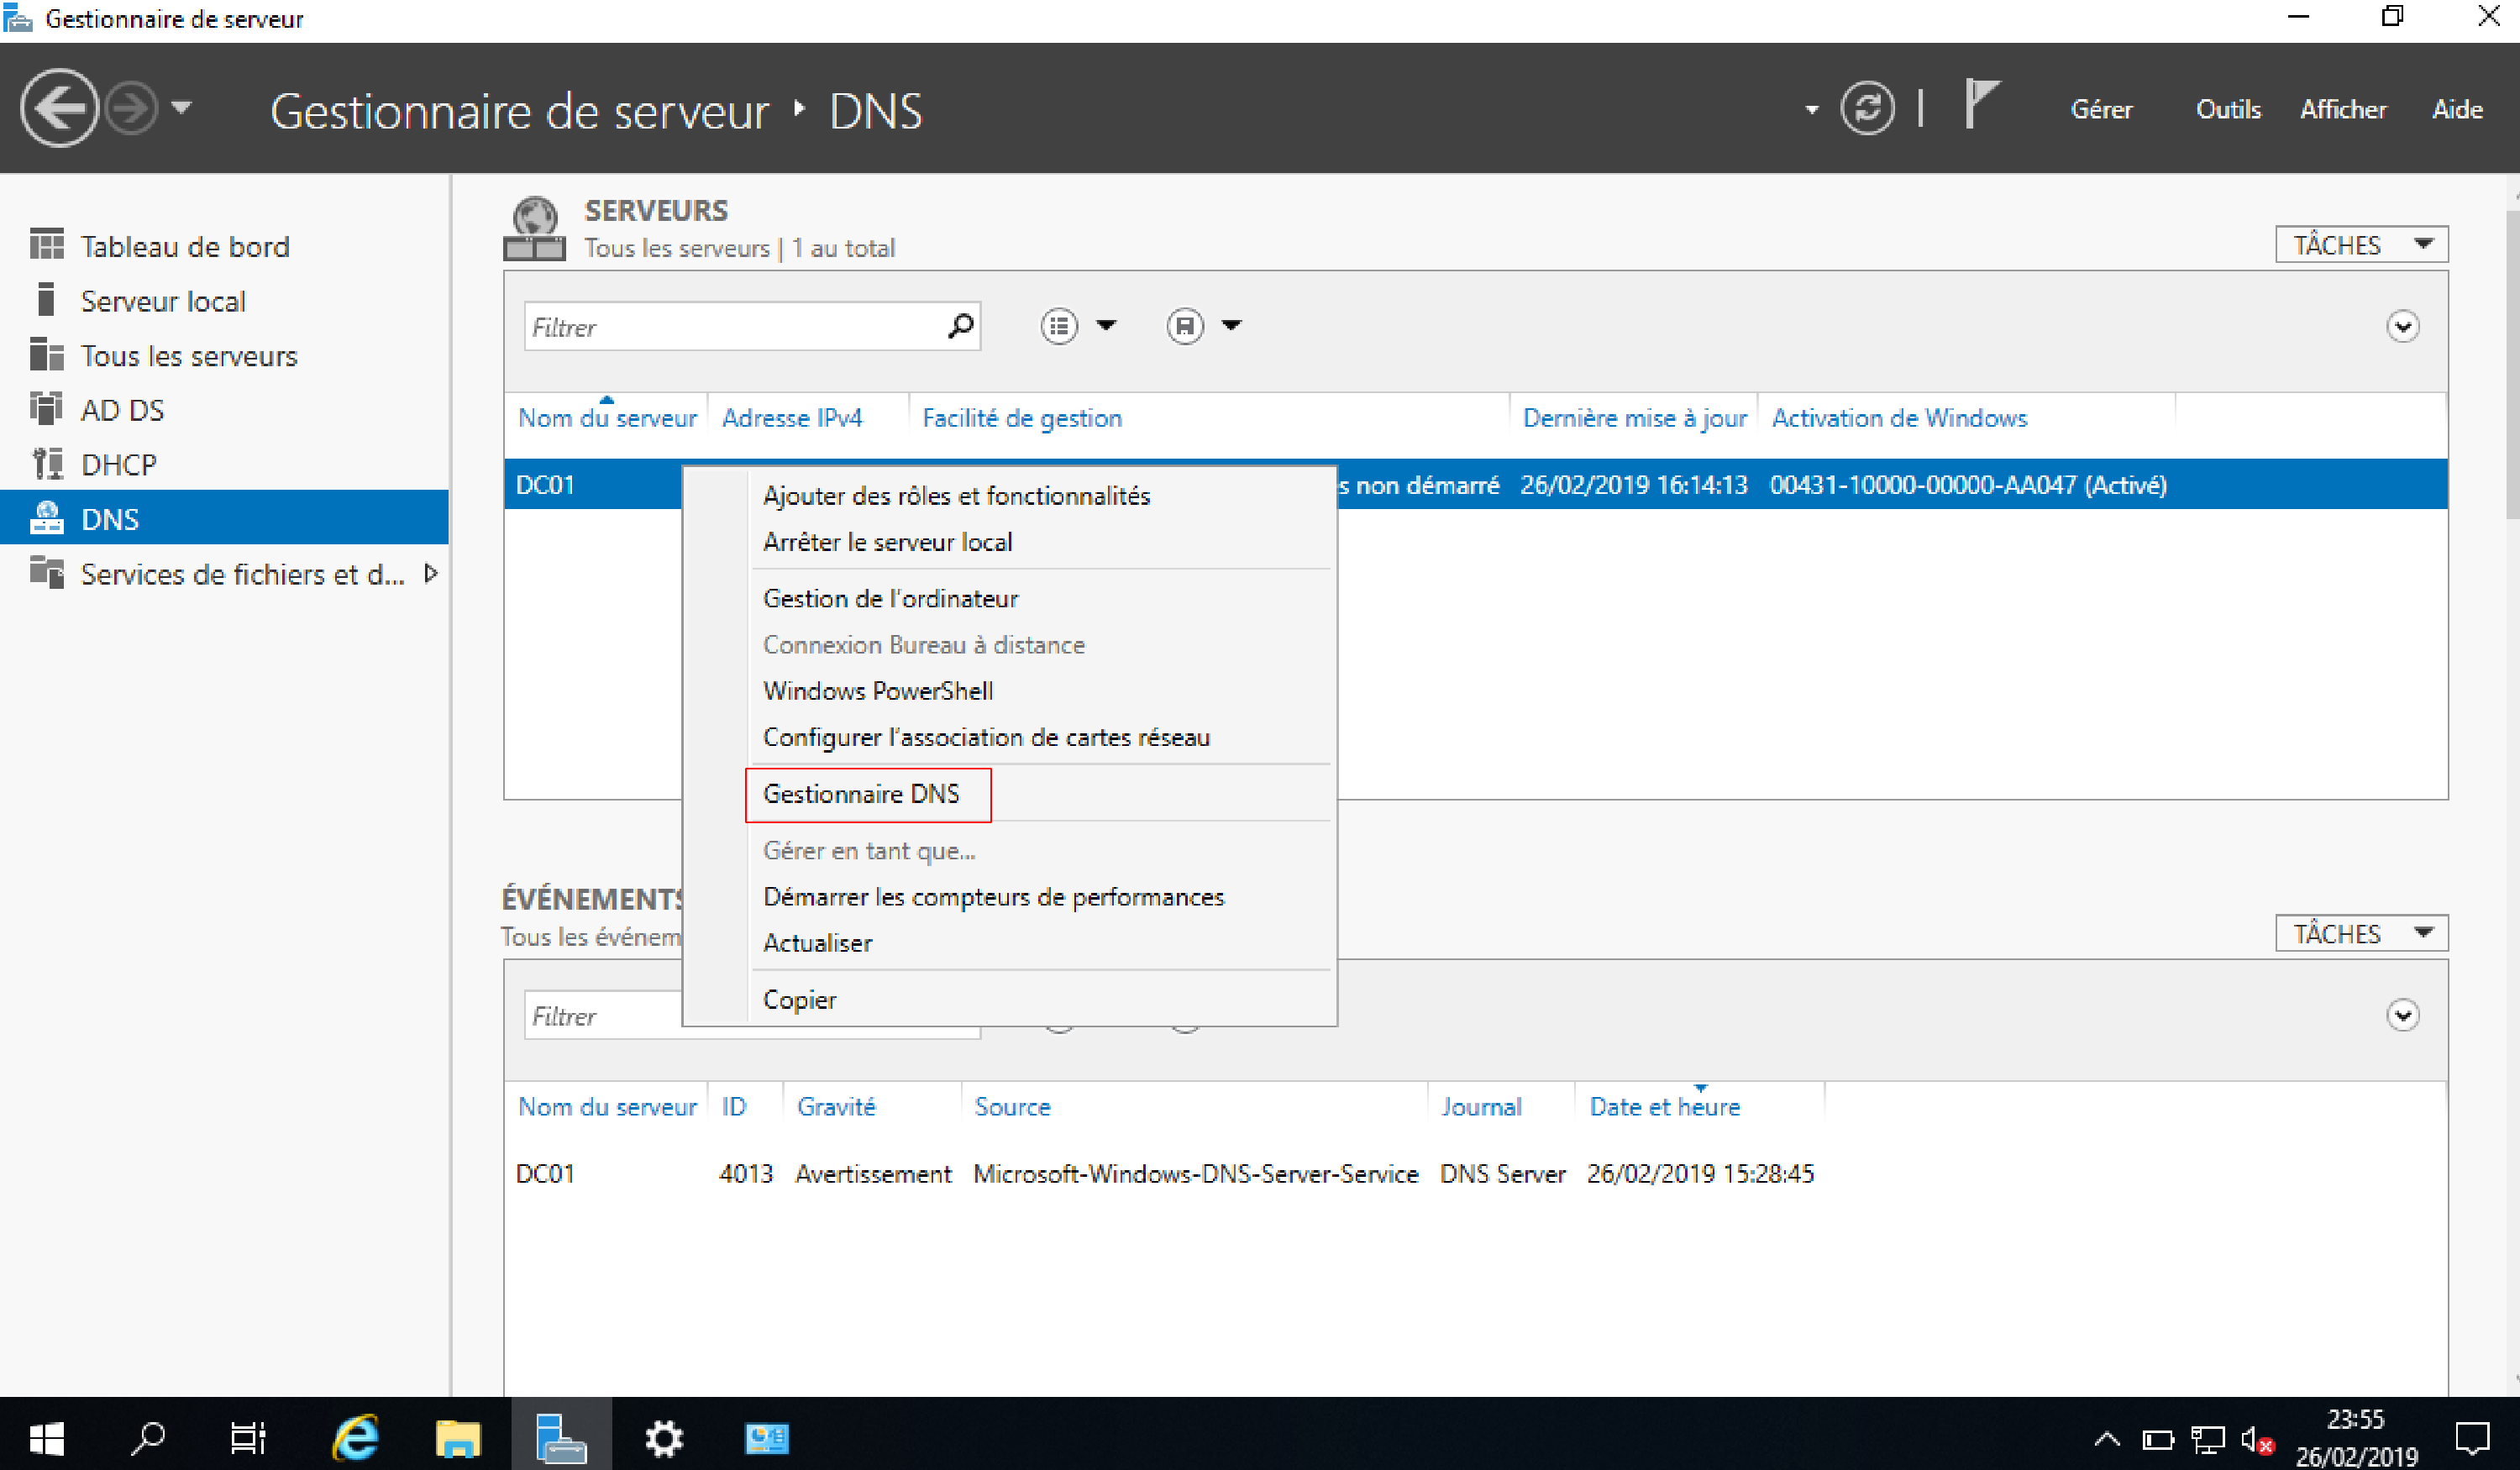
\includegraphics[scale=0.5]{WS_Screenshots/49.png}
		\label{Funcs_WinS/21}
	\end{center}
\end{figure}
\FloatBarrier 

\begin{figure}[h!]
	\begin{center}
		\caption{Modification des redirecteurs DNS de windows server}
		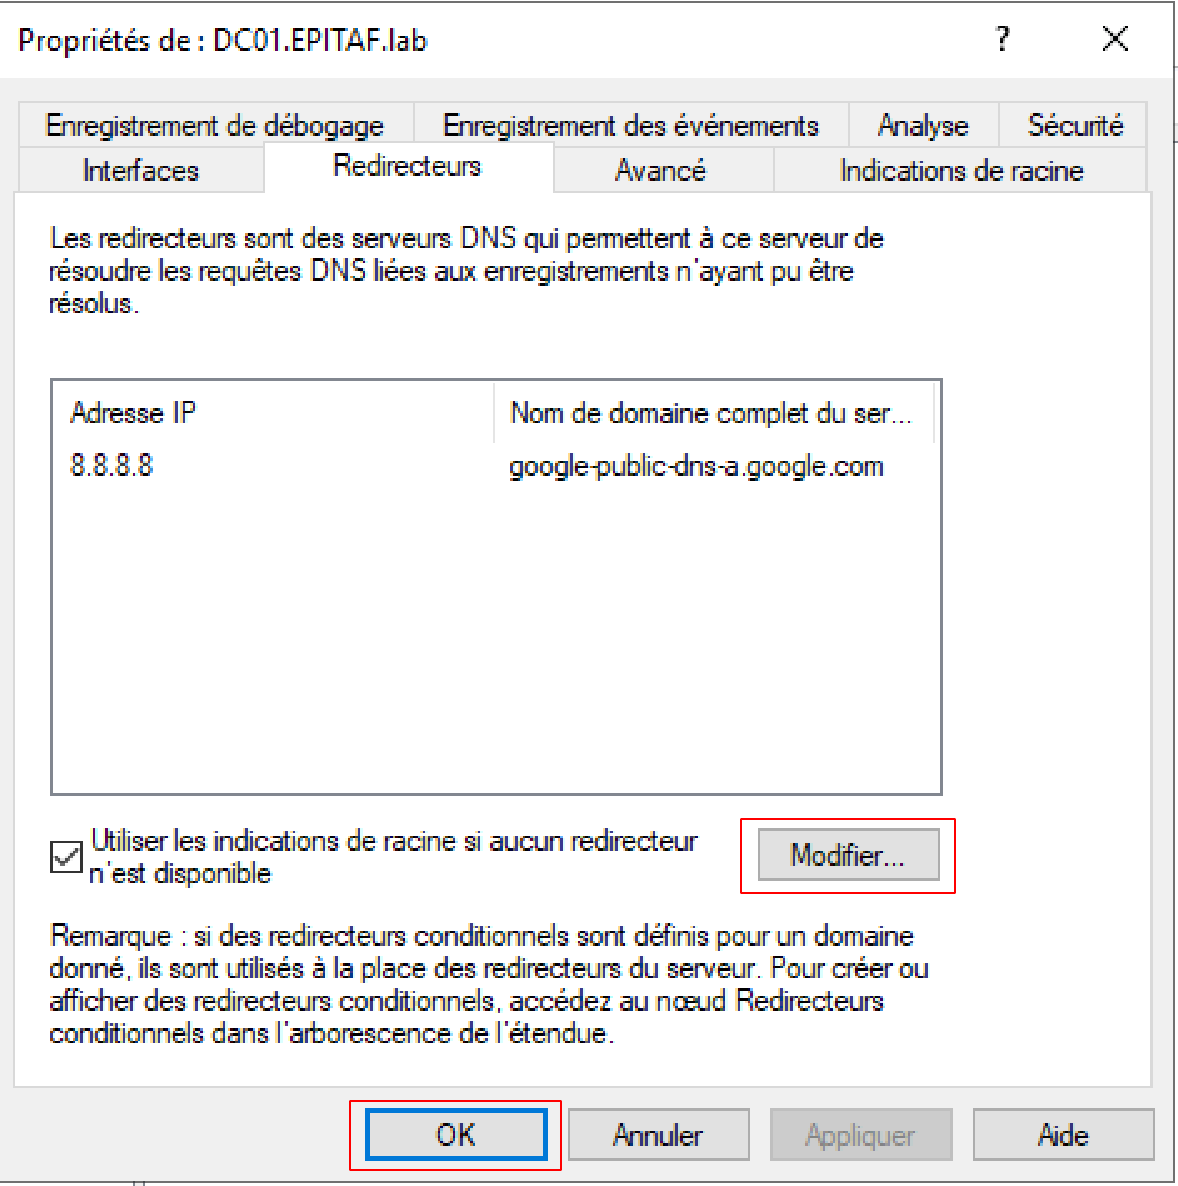
\includegraphics[scale=0.8]{WS_Screenshots/50.png}
		\label{Funcs_WinS/22}
	\end{center}
\end{figure}
\FloatBarrier

\begin{figure}[h!]
	\begin{center}
		\caption{Ajout du serveur DNS de windows server}
		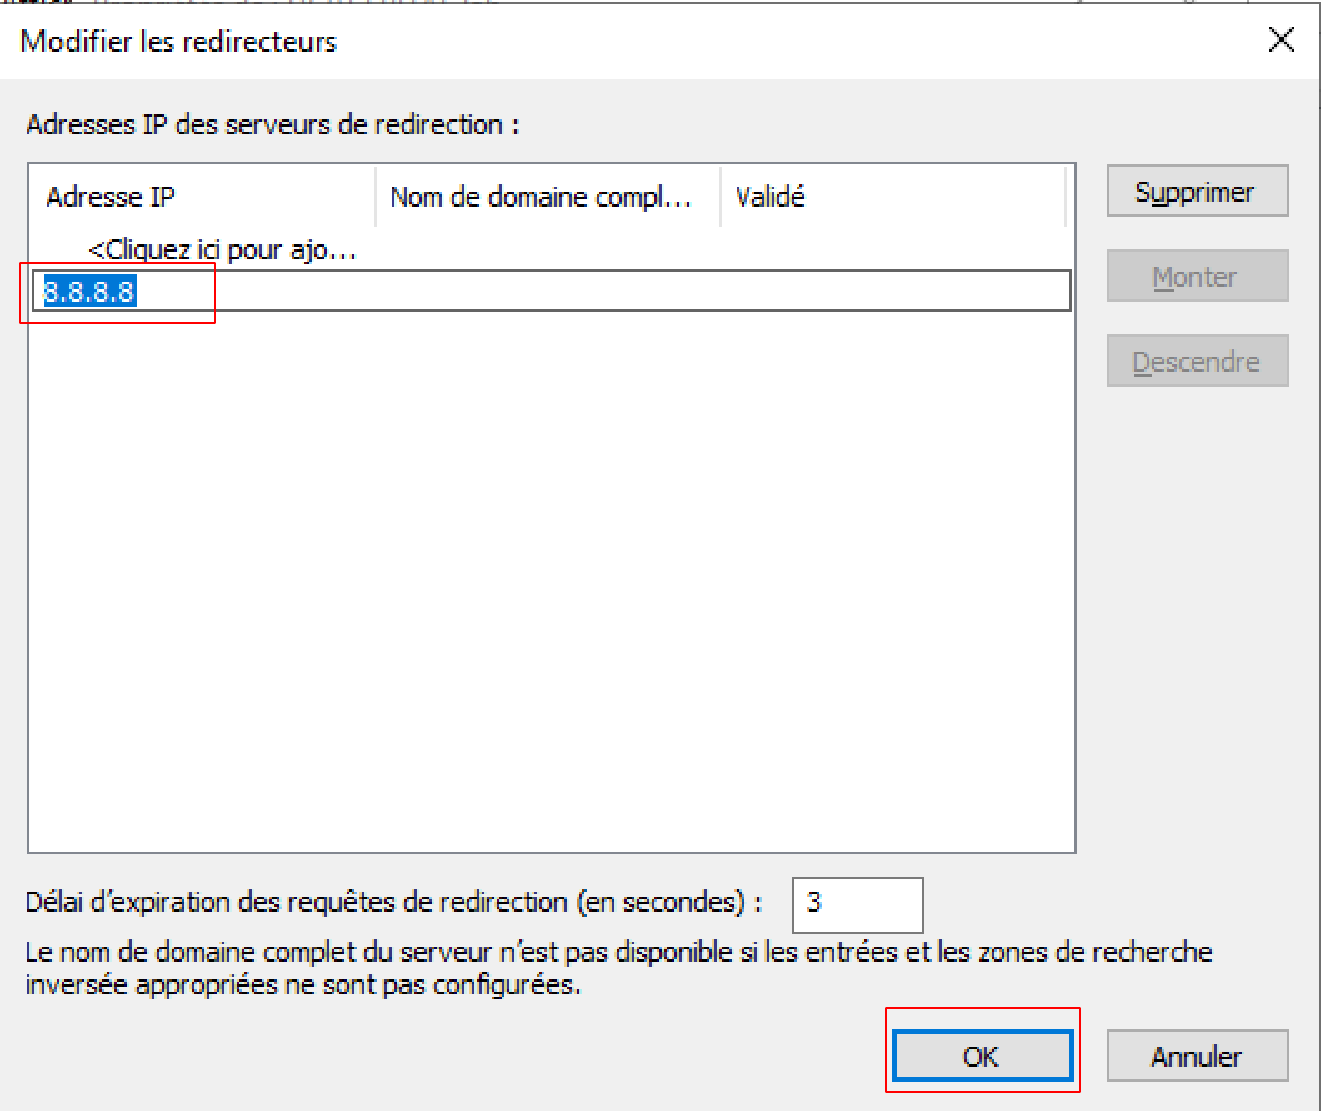
\includegraphics[scale=0.7]{WS_Screenshots/51.png}
		\label{Funcs_WinS/23}
	\end{center}
\end{figure}
\FloatBarrier

\begin{figure}[h!]
	\begin{center}
		\caption{Accepter le paramétrage du gestionnaire DNS de windows server}
		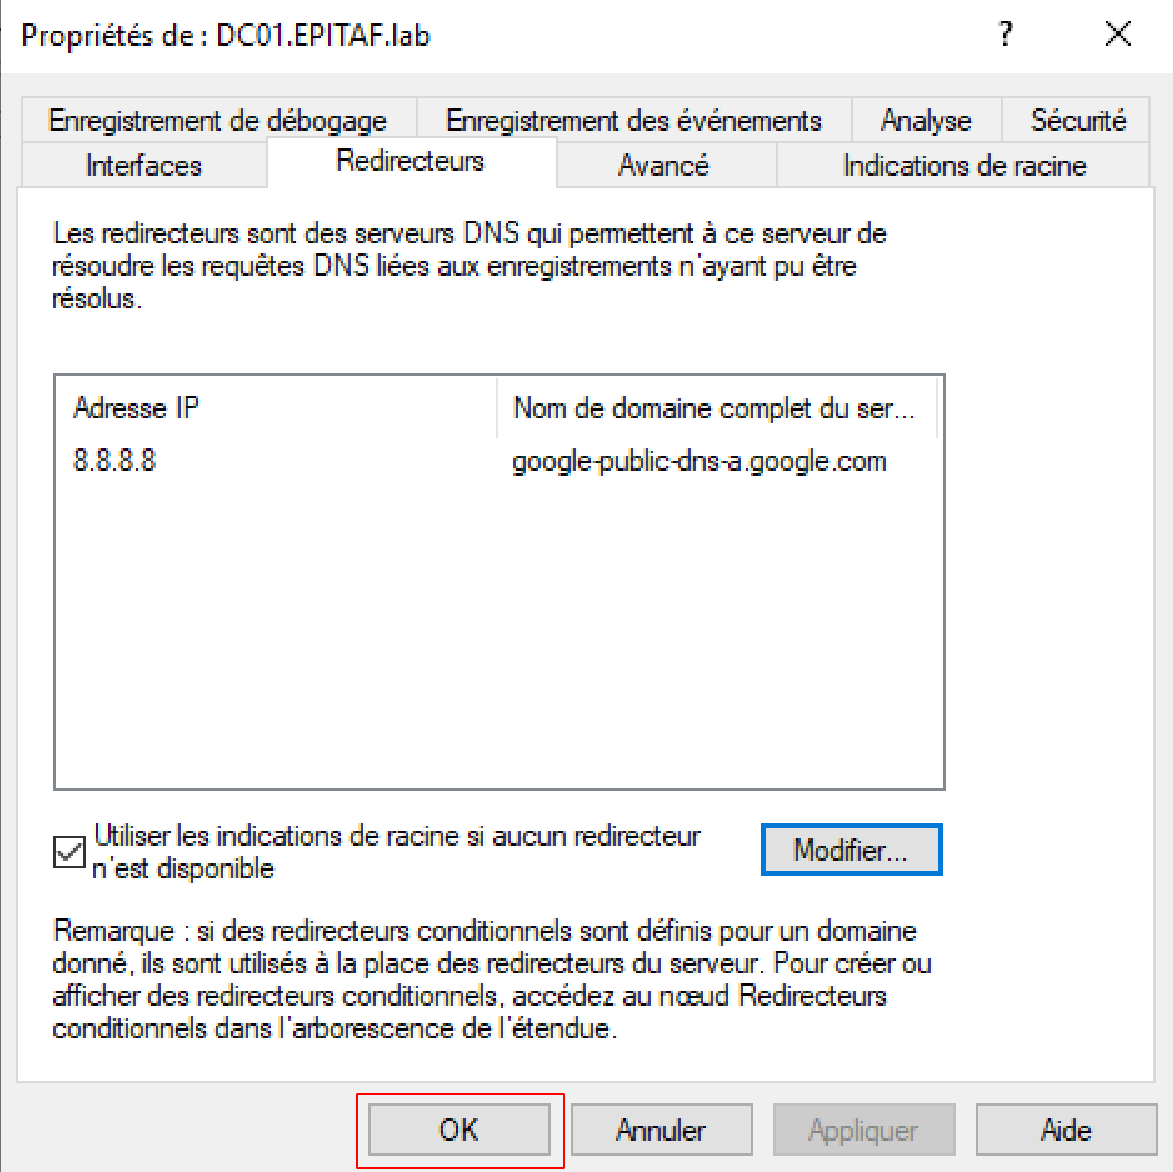
\includegraphics[scale=0.8]{WS_Screenshots/52.png}
		\label{Funcs_WinS/24}
	\end{center}
\end{figure}
\FloatBarrier

\subsection{Création des GPO}
Les deux sections suivantes permettent de créer deux gpo :
\begin{itemize}
    \item Une pour les mots de passe;
    \item Une autre pour les règles de pare-feu de Windows Server.
\end{itemize}
\subsubsection{GPO sur les mots de passe}
Le but est d'obtenir une gpo sur les mots de passe, telle que :
\begin{itemize}
    \item Le mot de passe doit être renouvelé tous les 42 jours;
    \item Le mot de passe doit être complexe;
    \item Le mot de passe doit faire au minimum 12 caractère;
    \item Le mot de passe ne peut pas être réversible.
\end{itemize}


Pour ce faire, il faut :
\begin{itemize}
    \item Cliquer sur \textbf{Group Policy Management} de l'onglet \textbf{Tools} (figure \ref{WS_Screenshots/gpo_0});
    \item Dérouler le menu \textbf{Forest: EPITAF.lab} : \texttt{Forest: EPITAF.lab -> Domains -> Group Policy Objects}, cliquer droit sur \textit{Group Policy Objects} puis cliquer sur \textit{New} (figure \ref{WS_Screenshots/gpo_1});
    \item Nommer la GPO \textit{Password Policy}, cliquer sur \textit{OK} (figure \ref{WS_Screenshots/gpo_2});
    \item Cliquer droit sur \textit{Password Policy}, cliquer ensuite sur \textit{Edit...} (figure \ref{WS_Screenshots/gpo_3});
    \item Cliquer sur \textit{Password Policy} (figure \ref{WS_Screenshots/gpo_4});
    \item Cliquer droit sur \textit{Maximum password age} puis cliquer sur \textit{Properties} (figure \ref{WS_Screenshots/gpo_5});
    \item Cocher la case, cliquer sur \textit{OK} (figure \ref{WS_Screenshots/gpo_6});
    \item Accepter le paramétrage proposé (figure \ref{WS_Screenshots/gpo_7});
    \item Cliquer droit sur \textit{Minimum password length} puis cliquer sur \textit{Properties} (figure \ref{WS_Screenshots/gpo_8});
    \item Cocher la case, mettre comme valeur \texttt{12}, cliquer sur \textit{OK} (figure \ref{WS_Screenshots/gpo_9});
    \item Cliquer droit sur \textit{Password must meet complexity requirements} puis cliquer sur \textit{Properties} (figure \ref{WS_Screenshots/gpo_10});
    \item Cocher la case, cliquer sur \textit{Enabled}, cliquer sur \textit{OK} (figure \ref{WS_Screenshots/gpo_11});
    \item Cliquer droit sur \textit{Store passwords using reversible encryption} puis cliquer sur \textit{Properties} (figure \ref{WS_Screenshots/gpo_12});
    \item Cocher la case, cliquer sur \textit{Disabled}, cliquer sur \textit{OK} (figure \ref{WS_Screenshots/gpo_13}).
\end{itemize}

\begin{figure}[h!]
	\begin{center}
		\caption{Accès au gestionnaire de politique de groupe de Windows Server}
		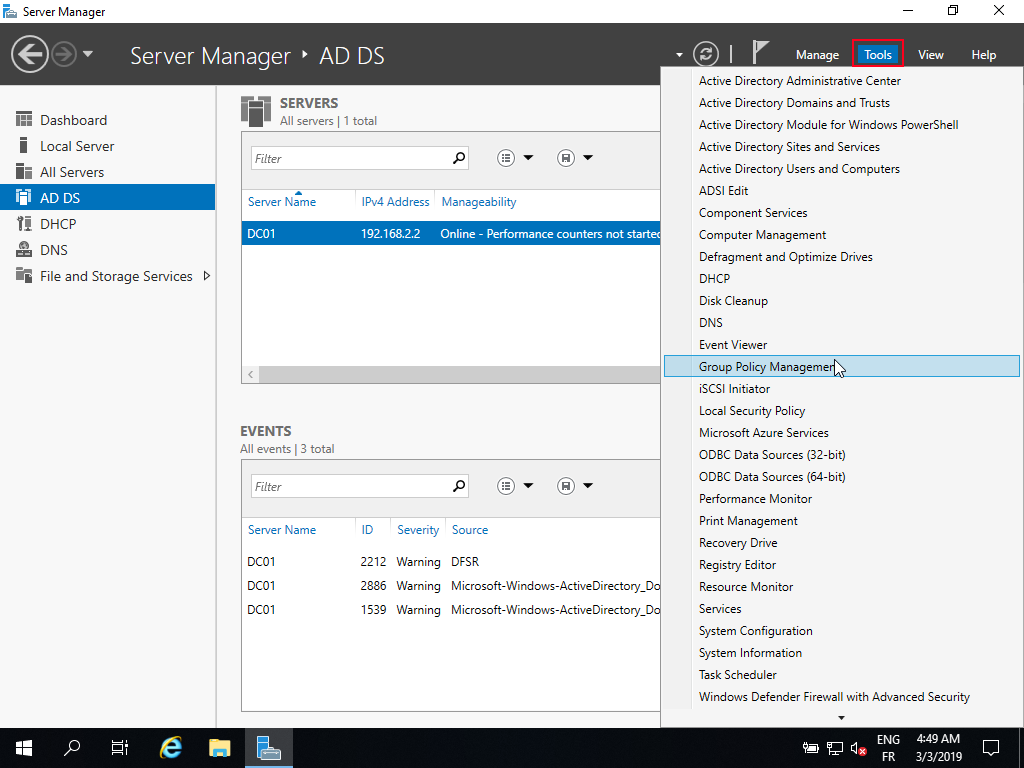
\includegraphics[scale=0.5]{WS_Screenshots/gpo_0.png}
		\label{WS_Screenshots/gpo_0}
	\end{center}
\end{figure}
\FloatBarrier 

\begin{figure}[h!]
	\begin{center}
		\caption{Création d'un nouvel object de politique de groupe sur Windows Server}
		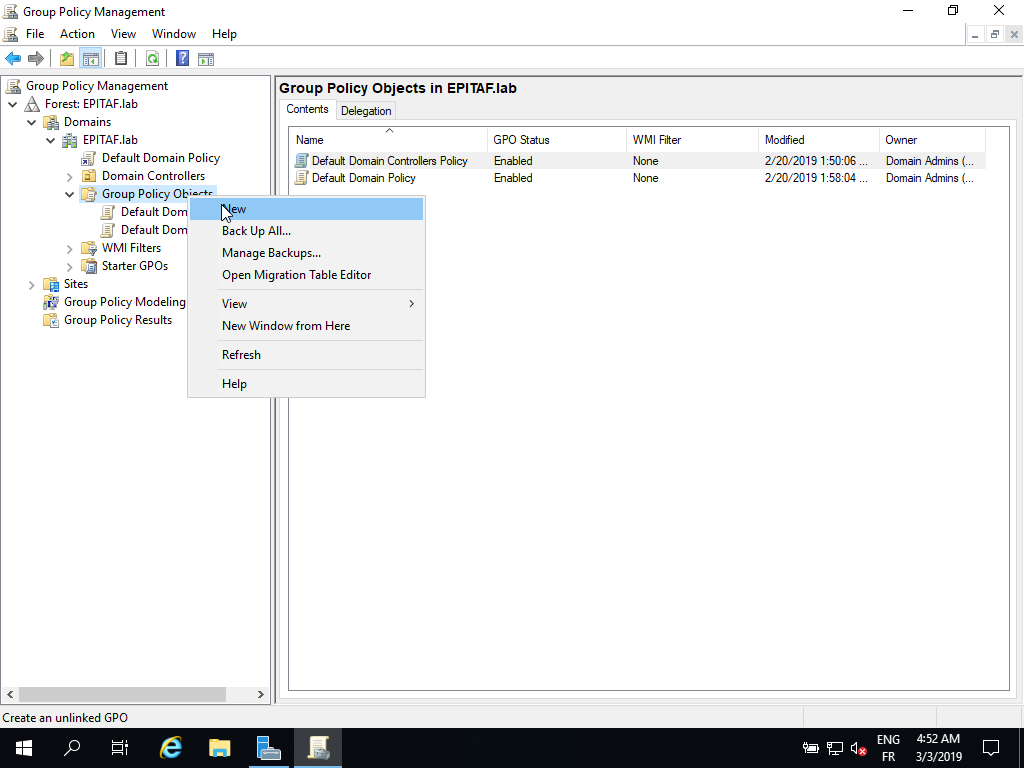
\includegraphics[scale=0.5]{WS_Screenshots/gpo_1.png}
		\label{WS_Screenshots/gpo_1}
	\end{center}
\end{figure}
\FloatBarrier 
    

\begin{figure}[h!]
	\begin{center}
		\caption{Attribution du nom de la gpo sur les mots de passe de Windows Server}
		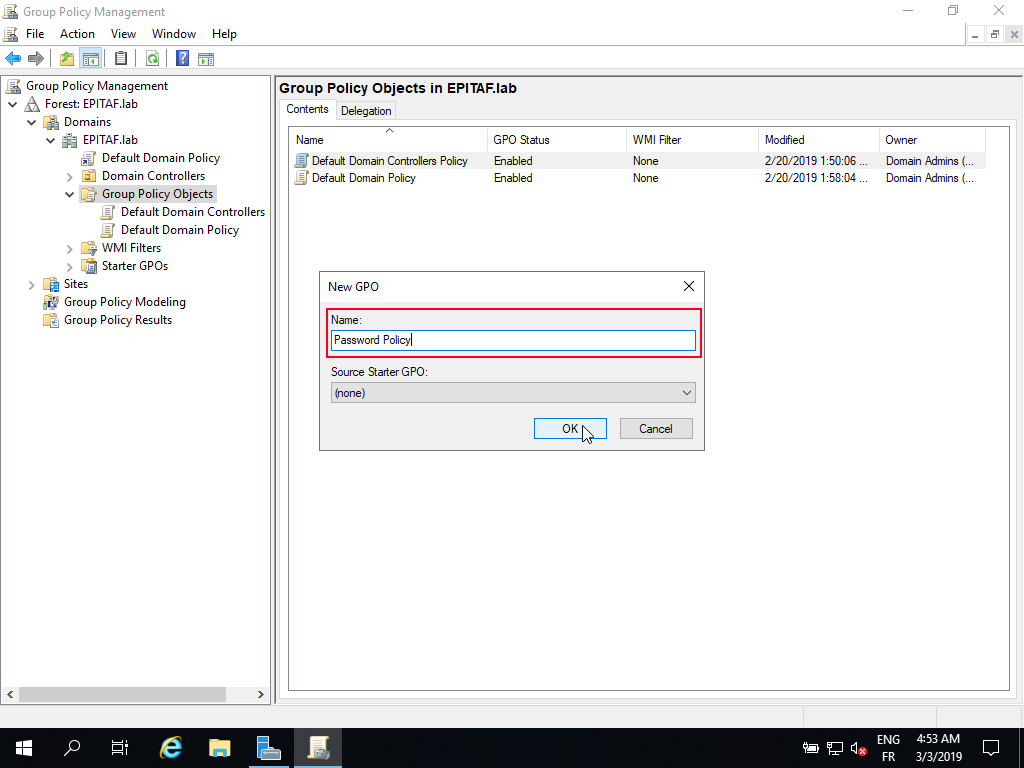
\includegraphics[scale=0.5]{WS_Screenshots/gpo_2.png}
		\label{WS_Screenshots/gpo_2}
	\end{center}
\end{figure}
\FloatBarrier 
    

\begin{figure}[h!]
	\begin{center}
		\caption{Modification de la gpo sur les mots de passe de Windows Server}
		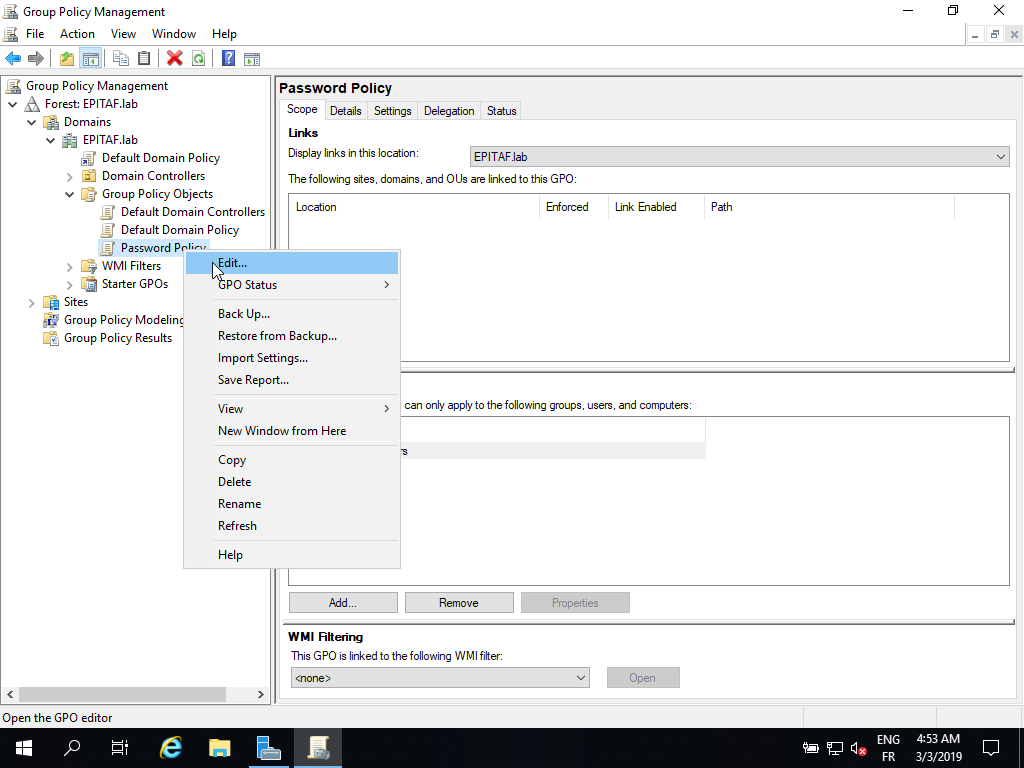
\includegraphics[scale=0.5]{WS_Screenshots/gpo_3.png}
		\label{WS_Screenshots/gpo_3}
	\end{center}
\end{figure}
\FloatBarrier 
    

\begin{figure}[h!]
	\begin{center}
		\caption{Accès à la politique de la gpo sur les mots de passe de Windows Server}
		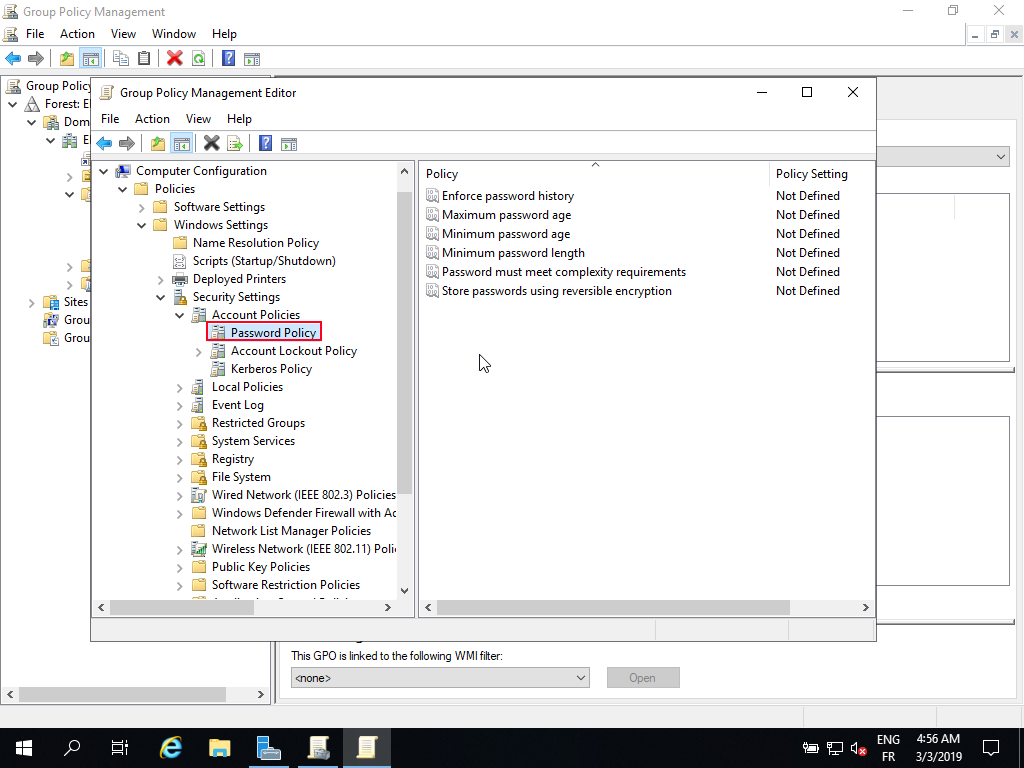
\includegraphics[scale=0.5]{WS_Screenshots/gpo_4.png}
		\label{WS_Screenshots/gpo_4}
	\end{center}
\end{figure}
\FloatBarrier 
    

\begin{figure}[h!]
	\begin{center}
		\caption{Accès aux propriétés de durée maximum d'un mot de passe sur Windows Server}
		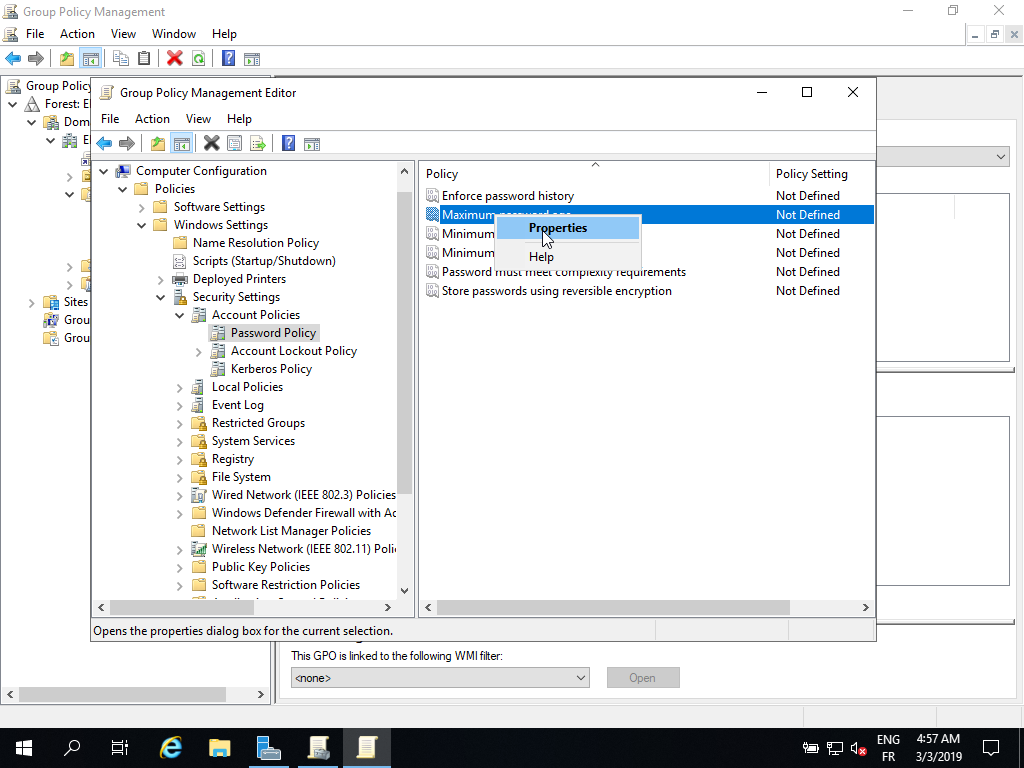
\includegraphics[scale=0.5]{WS_Screenshots/gpo_5.png}
		\label{WS_Screenshots/gpo_5}
	\end{center}
\end{figure}
\FloatBarrier 
    

\begin{figure}[h!]
	\begin{center}
		\caption{Activation et validation de la politique de durée maximum des mots de passe sur Windows Server}
		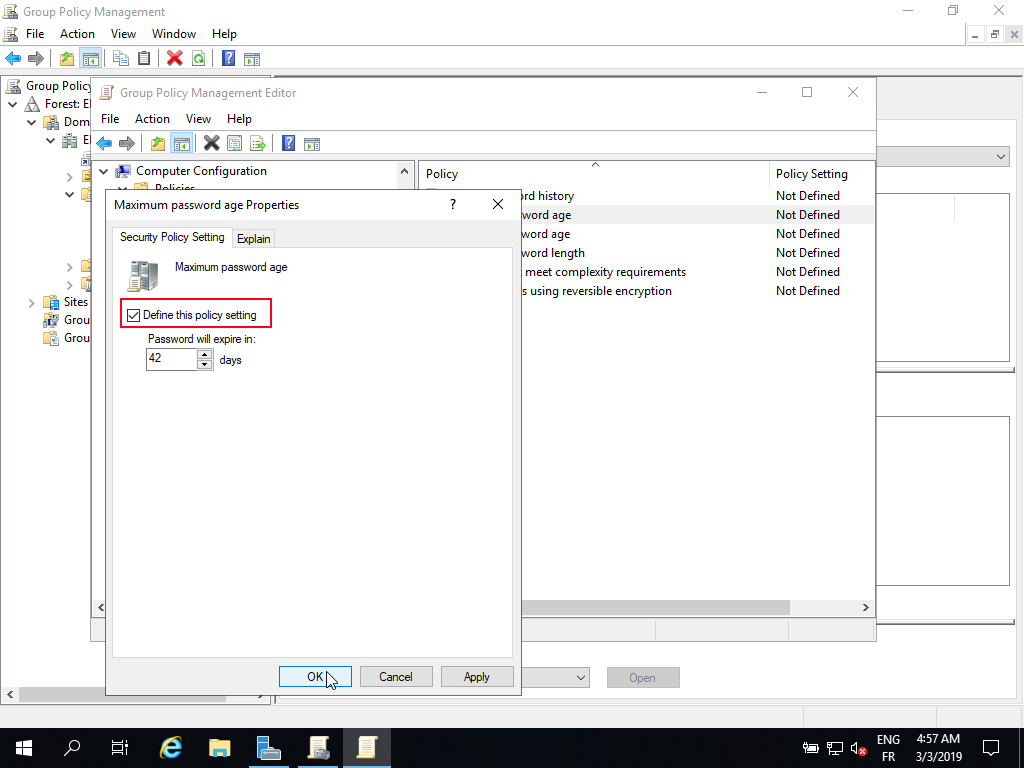
\includegraphics[scale=0.5]{WS_Screenshots/gpo_6.png}
		\label{WS_Screenshots/gpo_6}
	\end{center}
\end{figure}
\FloatBarrier 
    

\begin{figure}[h!]
	\begin{center}
		\caption{Validation du paramétrage par défaut sur Windows Server}
		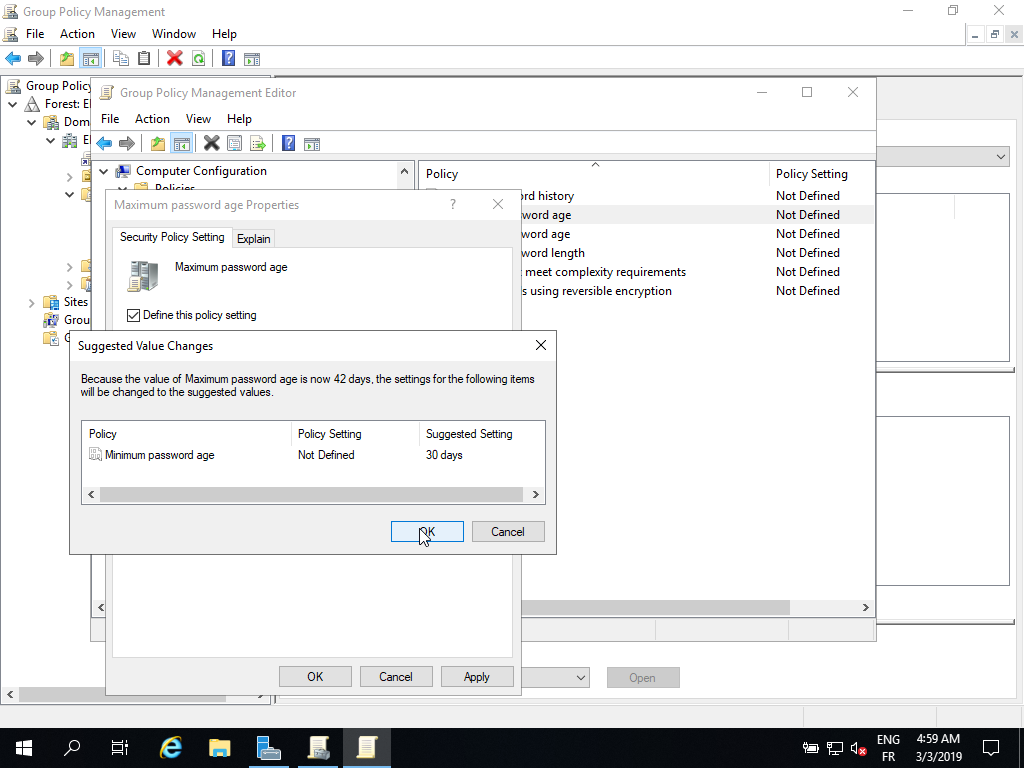
\includegraphics[scale=0.5]{WS_Screenshots/gpo_7.png}
		\label{WS_Screenshots/gpo_7}
	\end{center}
\end{figure}
\FloatBarrier 
    

\begin{figure}[h!]
	\begin{center}
		\caption{Accès aux propriétés de longueur minimale d'un mot de passe sur Windows Server}
		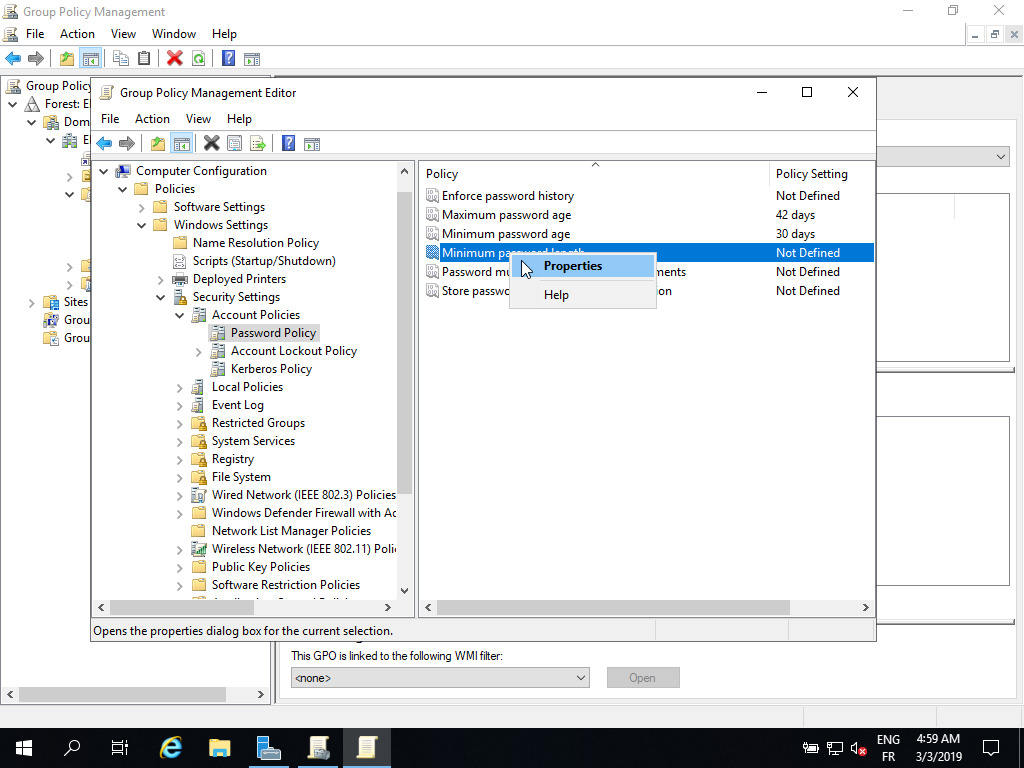
\includegraphics[scale=0.5]{WS_Screenshots/gpo_8.png}
		\label{WS_Screenshots/gpo_8}
	\end{center}
\end{figure}
\FloatBarrier 
    

\begin{figure}[h!]
	\begin{center}
		\caption{Activation et validation de longueur minimale d'un mot de passe sur Windows Server}
		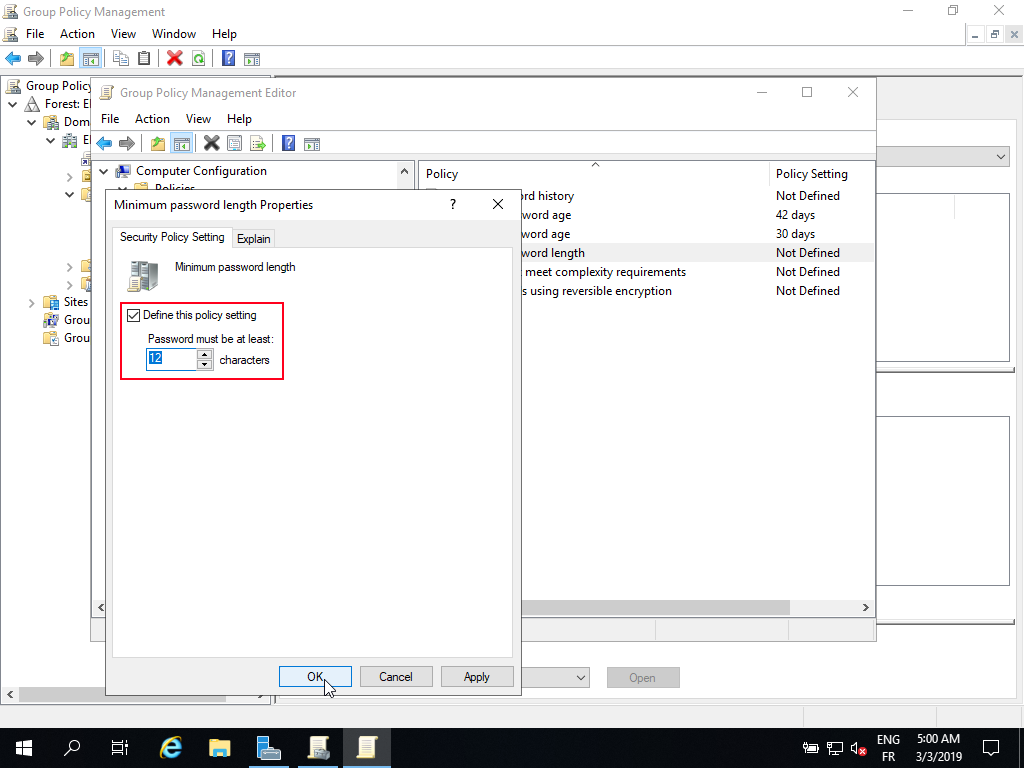
\includegraphics[scale=0.5]{WS_Screenshots/gpo_9.png}
		\label{WS_Screenshots/gpo_9}
	\end{center}
\end{figure}
\FloatBarrier 
    

\begin{figure}[h!]
	\begin{center}
		\caption{Accès aux propriétés de complexité d'un mot de passe sur Windows Server}
		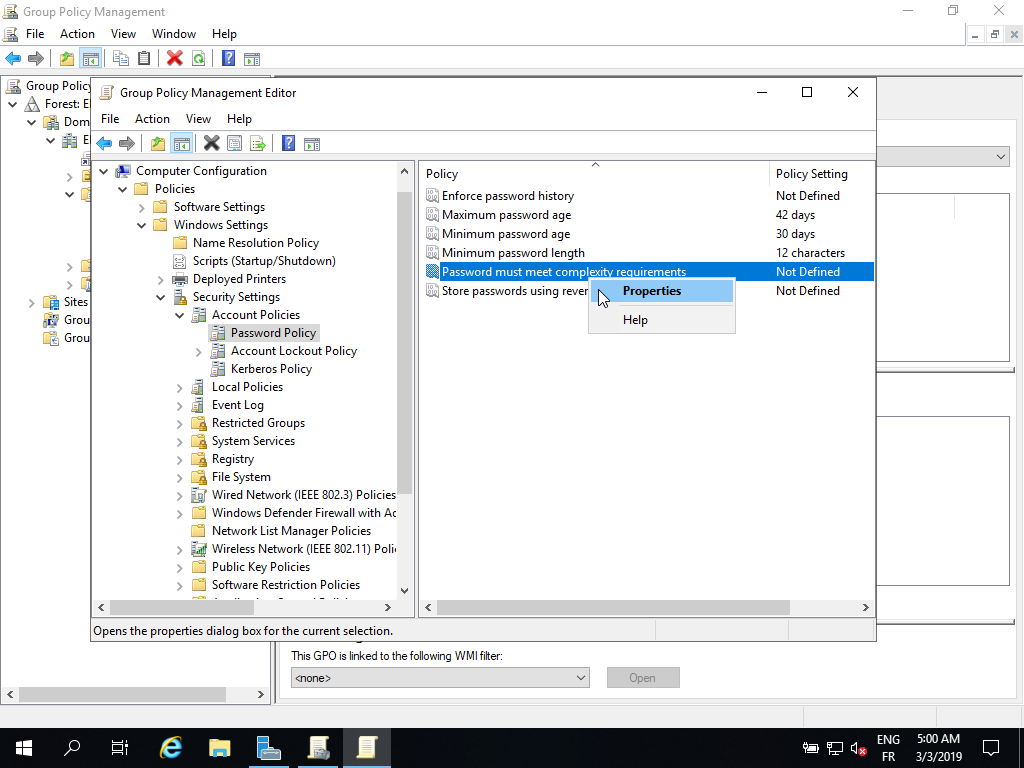
\includegraphics[scale=0.5]{WS_Screenshots/gpo_10.png}
		\label{WS_Screenshots/gpo_10}
	\end{center}
\end{figure}
\FloatBarrier 
    

\begin{figure}[h!]
	\begin{center}
		\caption{Activation et validation de complexité d'un mot de passe sur Windows Server}
		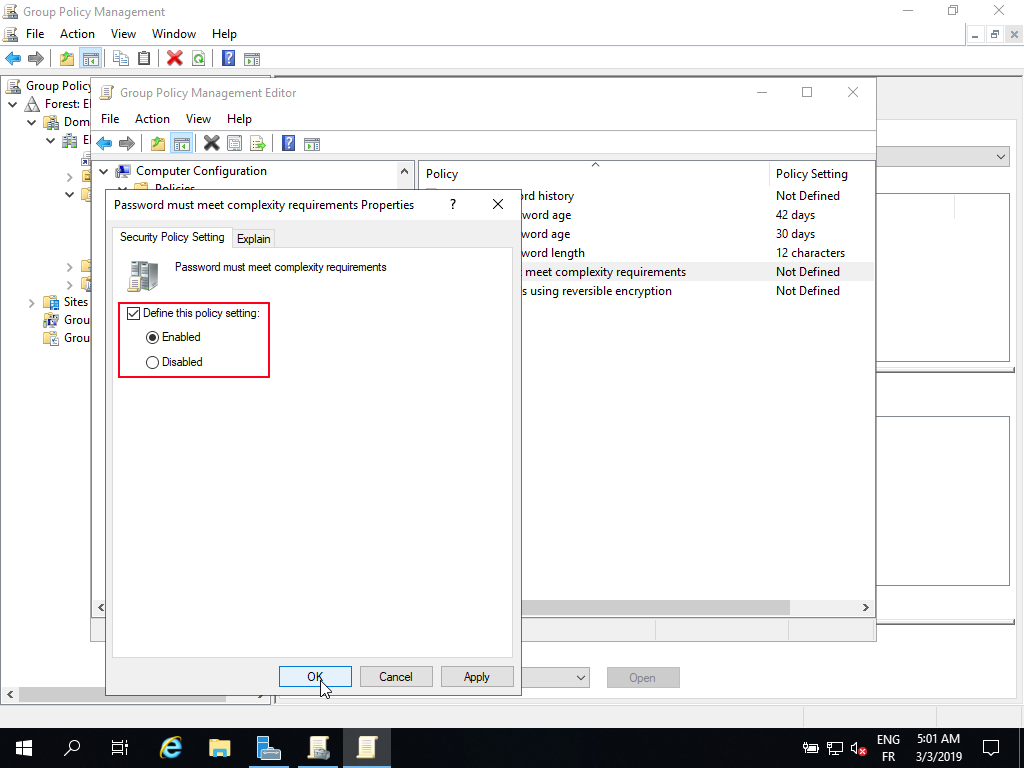
\includegraphics[scale=0.5]{WS_Screenshots/gpo_11.png}
		\label{WS_Screenshots/gpo_11}
	\end{center}
\end{figure}
\FloatBarrier 
    

\begin{figure}[h!]
	\begin{center}
		\caption{Accès aux propriétés de réversibilité d'un mot de passe sur Windows Server}
		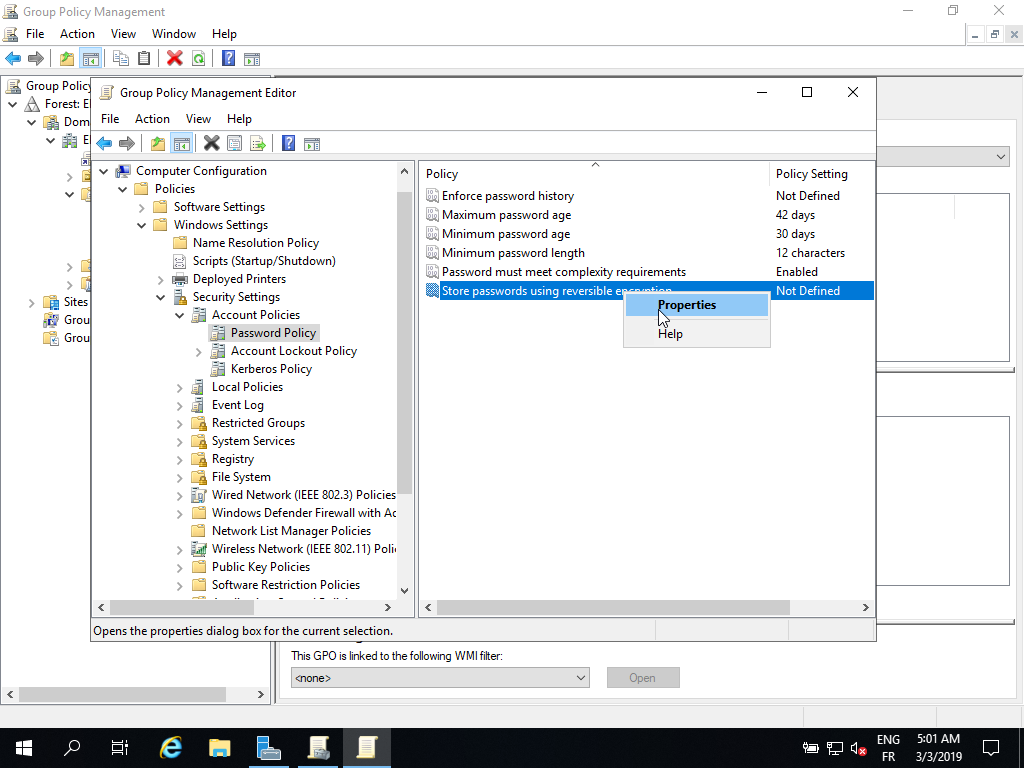
\includegraphics[scale=0.5]{WS_Screenshots/gpo_12.png}
		\label{WS_Screenshots/gpo_12}
	\end{center}
\end{figure}
\FloatBarrier 
    

\begin{figure}[h!]
	\begin{center}
		\caption{Désactivation et validation du paramétrage de réversibilité d'un mot de passe sur Windows Server}
		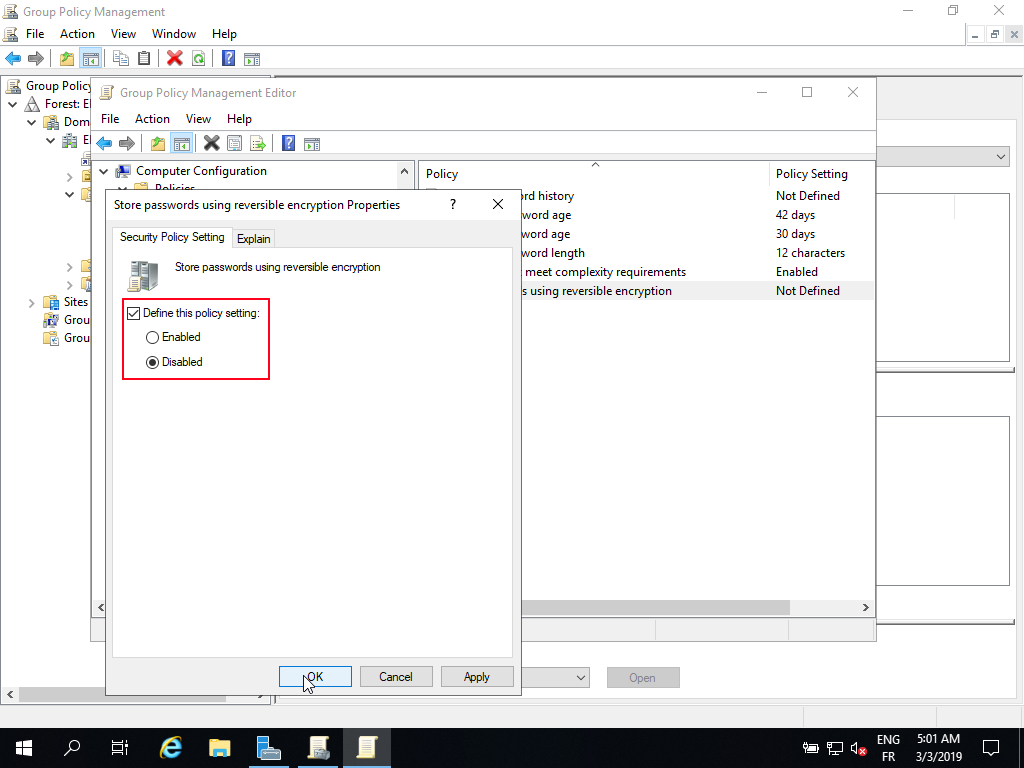
\includegraphics[scale=0.5]{WS_Screenshots/gpo_13.png}
		\label{WS_Screenshots/gpo_13}
	\end{center}
\end{figure}
\FloatBarrier 
    
\subsubsection{GPO sur le pare-feu de Windows Server}

Le but est de bloquer le port 22 (SSH) via une gpo. \\
Pour ce faire, il faut:
\begin{itemize}
    \item Cliquer sur \textbf{Group Policy Management} de l'onglet \textbf{Tools} (figure \ref{WS_Screenshots/gpo_0});
    \item Dérouler le menu \textbf{Forest: EPITAF.lab} : \texttt{Forest: EPITAF.lab -> Domains -> Group Policy Objects}, cliquer droit sur \textit{Group Policy Objects} puis cliquer sur \textit{New} (figure \ref{WS_Screenshots/gpo_1});
    \item Nommer la GPO \textit{Firewall}, cliquer sur \textit{OK} (figure \ref{WS_Screenshots/gpo_14});
    \item Cliquer droit sur \textit{Firewall}, cliquer ensuite sur \textit{Edit...} (figure \ref{WS_Screenshots/gpo_15});
    \item Dérouler le menu \textbf{Windows Settings} : \texttt{Windows Settings -> Security Settings -> Windows Defender Firewall ... -> Windows Defender Firewall ...}, cliquer droit sur \textit{Inbound Rules} puis cliquer sur \textit{New Rule...} (figure \ref{WS_Screenshots/gpo_16});
    \item Cliquer sur \textit{Port} puis cliquer sur \textit{Next} (figure \ref{WS_Screenshots/gpo_17});
    \item Cliquer sur \textit{Specific local ports}, remplir par \texttt{22} puis cliquer sur \textit{next} (figure \ref{WS_Screenshots/gpo_18});
    \item Cliquer sur \textit{Block the connection} (figure \ref{WS_Screenshots/gpo_19});
    \item Cliquer sur \textit{Next} (figure \ref{WS_Screenshots/gpo_20});
    \item Remplir \textit{Name} par \texttt{NO SSH} puis cliquer sur \textit{Finish} (figure \ref{WS_Screenshots/gpo_21});
\end{itemize}

\begin{figure}[h!]
	\begin{center}
		\caption{Attribution du nom de la gpo sur le pare-feu de Windows Server}
		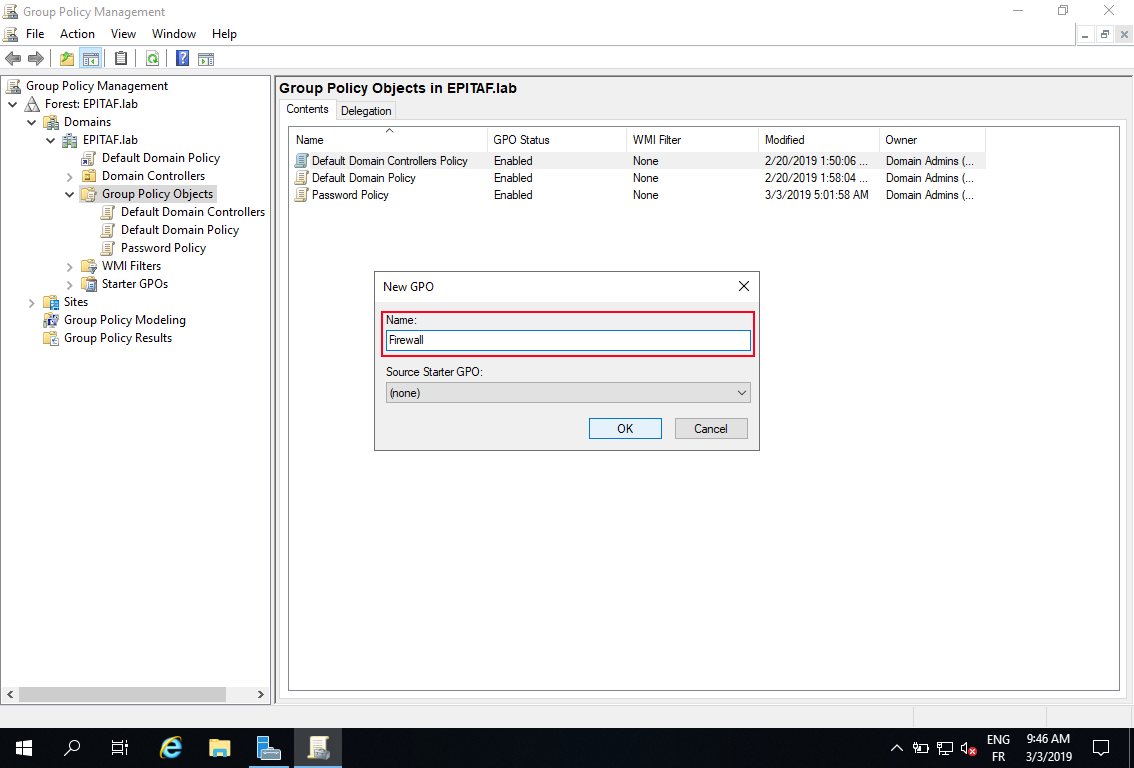
\includegraphics[scale=0.5]{WS_Screenshots/gpo_14.png}
		\label{WS_Screenshots/gpo_14}
	\end{center}
\end{figure}
\FloatBarrier 
    

\begin{figure}[h!]
	\begin{center}
		\caption{Modification de la gpo sur le pare-feu de Windows Server}
		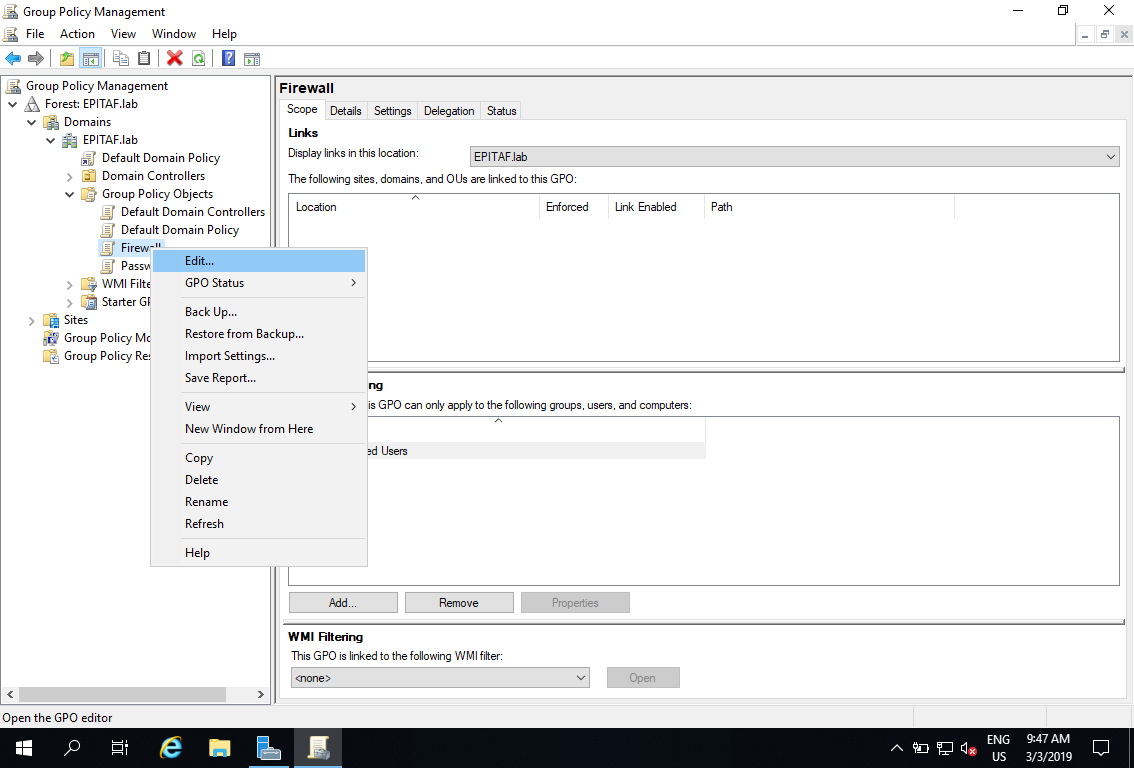
\includegraphics[scale=0.5]{WS_Screenshots/gpo_15.png}
		\label{WS_Screenshots/gpo_15}
	\end{center}
\end{figure}
\FloatBarrier 
    

\begin{figure}[h!]
	\begin{center}
		\caption{Création d'une règle du pare-feu de la gpo de Windows Server}
		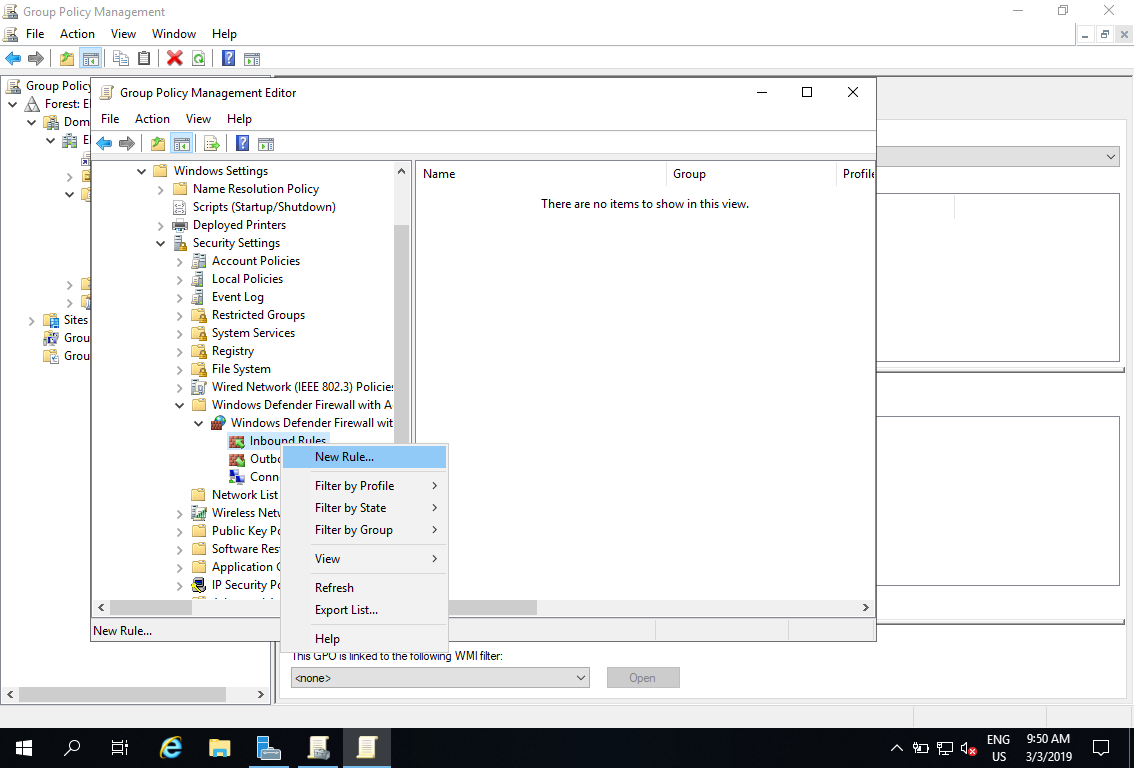
\includegraphics[scale=0.5]{WS_Screenshots/gpo_16.png}
		\label{WS_Screenshots/gpo_16}
	\end{center}
\end{figure}
\FloatBarrier 
    

\begin{figure}[h!]
	\begin{center}
		\caption{Choix du type de règle pour le pare-feu de Windows Server}
		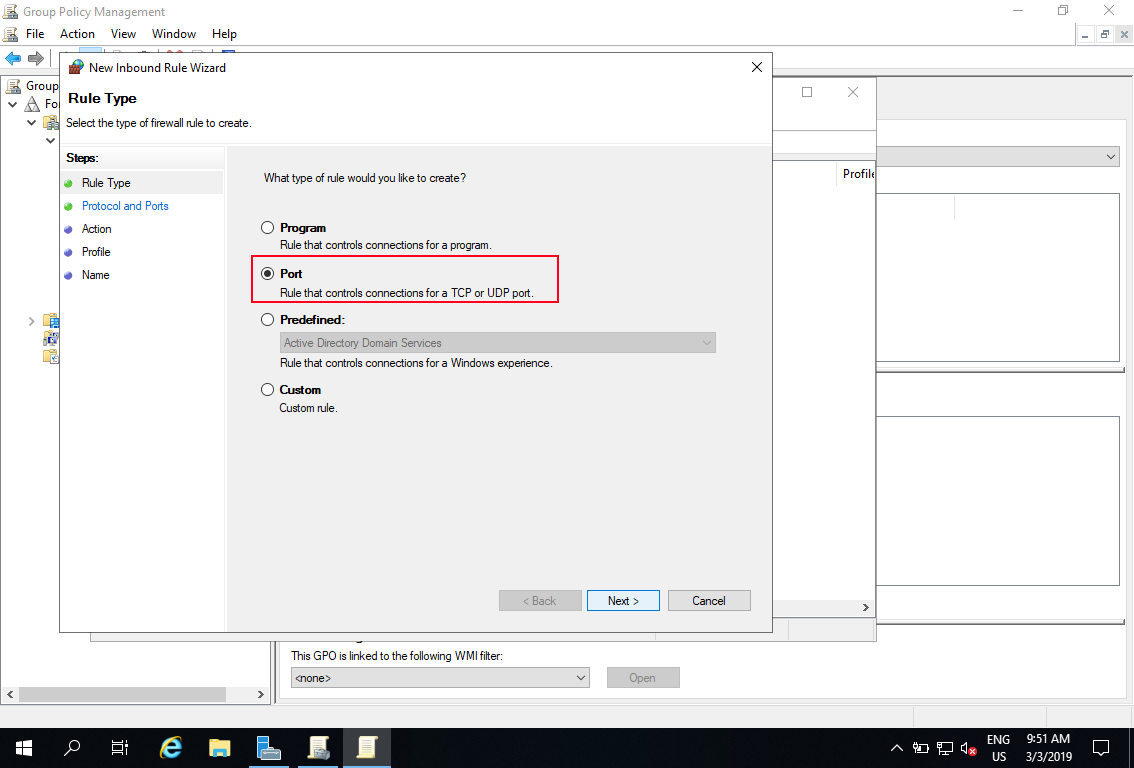
\includegraphics[scale=0.5]{WS_Screenshots/gpo_17.png}
		\label{WS_Screenshots/gpo_17}
	\end{center}
\end{figure}
\FloatBarrier 
    

\begin{figure}[h!]
	\begin{center}
		\caption{Choix des ports pour le pare-feu de Windows Server}
		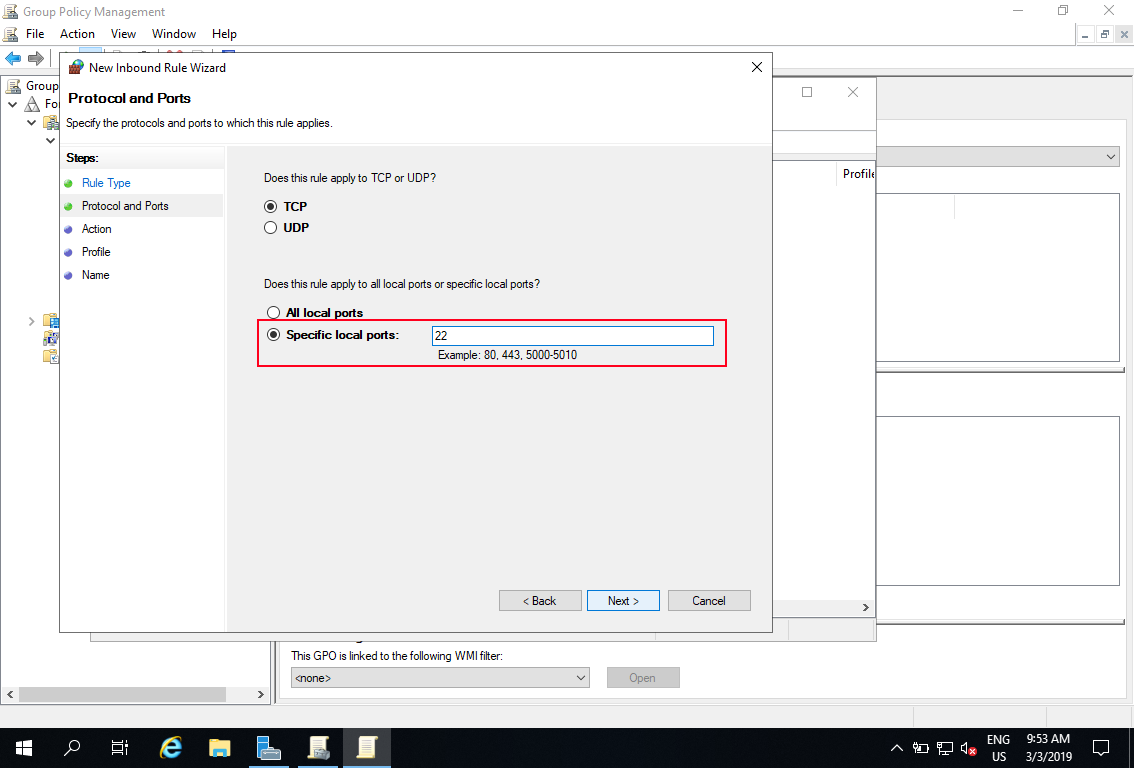
\includegraphics[scale=0.5]{WS_Screenshots/gpo_18.png}
		\label{WS_Screenshots/gpo_18}
	\end{center}
\end{figure}
\FloatBarrier 
    

\begin{figure}[h!]
	\begin{center}
		\caption{Blocage du port 22 de Windows Server}
		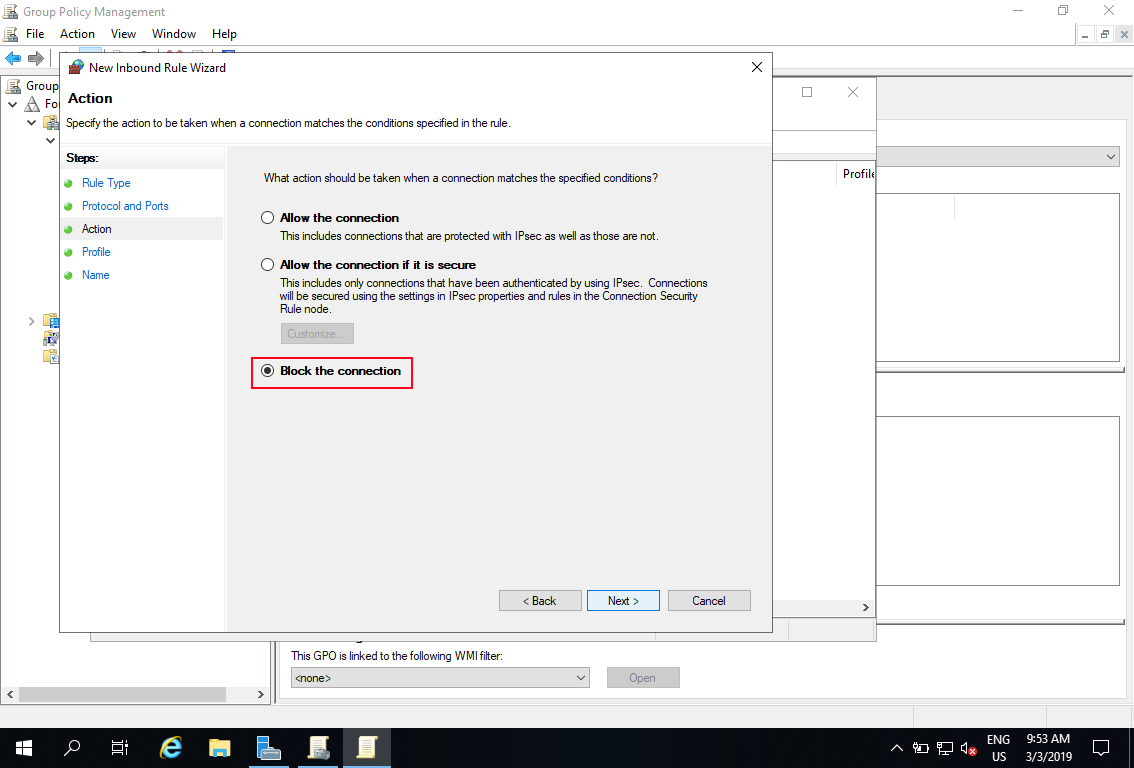
\includegraphics[scale=0.5]{WS_Screenshots/gpo_19.png}
		\label{WS_Screenshots/gpo_19}
	\end{center}
\end{figure}
\FloatBarrier 
    

\begin{figure}[h!]
	\begin{center}
		\caption{Sélection des profils concernés par la nouvelle règle sur Windows Server}
		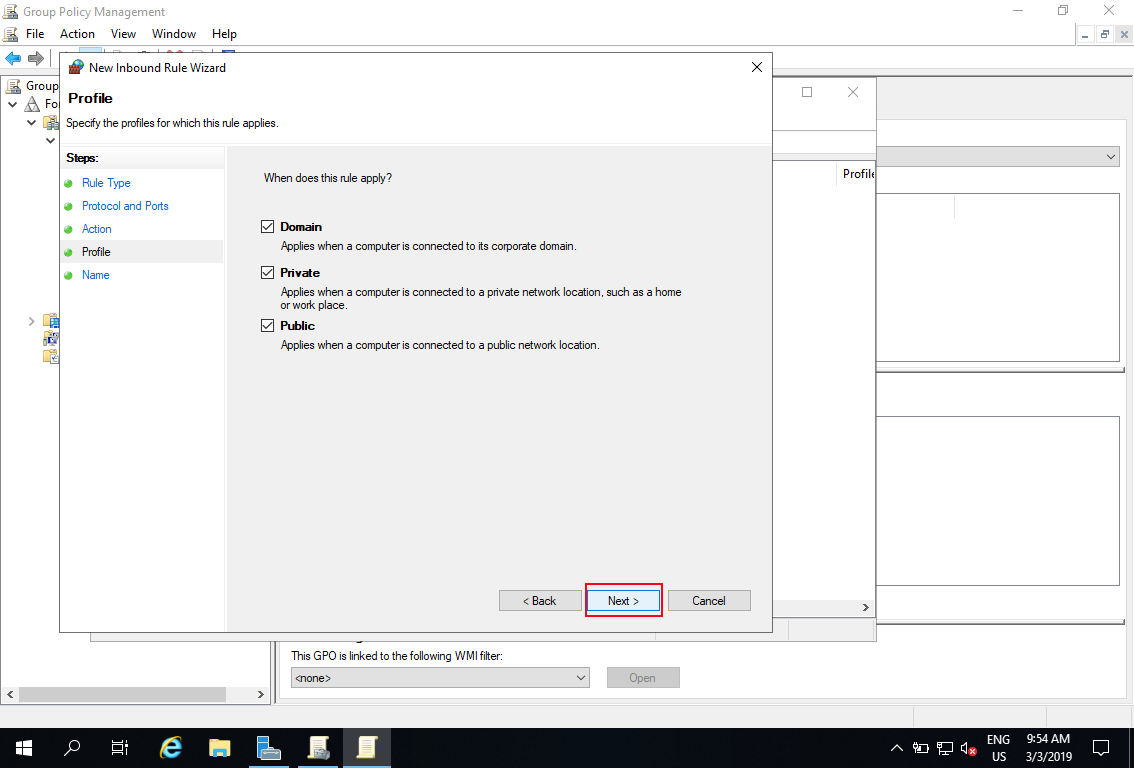
\includegraphics[scale=0.5]{WS_Screenshots/gpo_20.png}
		\label{WS_Screenshots/gpo_20}
	\end{center}
\end{figure}
\FloatBarrier 
    

\begin{figure}[h!]
	\begin{center}
		\caption{Nom et validation de la nouvelle règle sur Windows Server}
		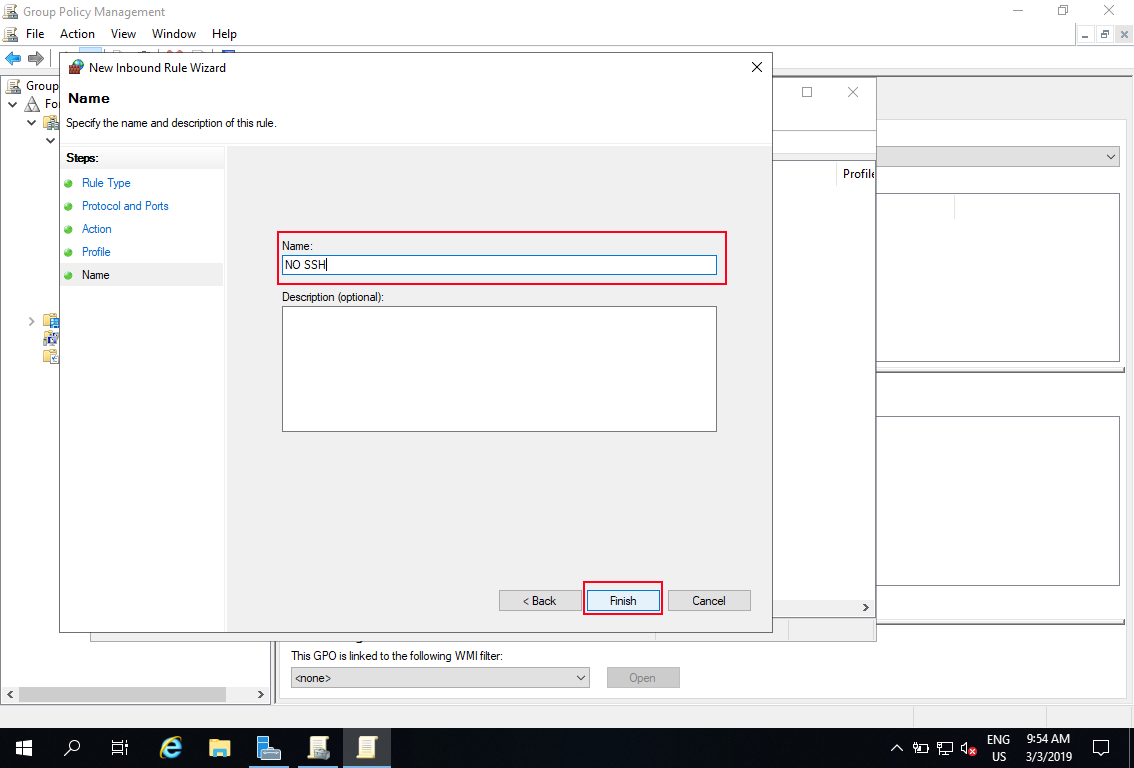
\includegraphics[scale=0.5]{WS_Screenshots/gpo_21.png}
		\label{WS_Screenshots/gpo_21}
	\end{center}
\end{figure}
\FloatBarrier